\documentclass[twoside]{article}
\setlength{\oddsidemargin}{0.25 in}
\setlength{\evensidemargin}{-0.25 in}
\setlength{\topmargin}{-0.6 in}
\setlength{\textwidth}{6.5 in}
\setlength{\textheight}{8.5 in}
\setlength{\headsep}{0.75 in}
\setlength{\parindent}{0 in}
\setlength{\parskip}{0.1 in}

%
% ADD PACKAGES here:
%

\usepackage{amsmath,amsfonts,amssymb,graphicx,mathtools,flexisym, hyperref, graphicx}
\graphicspath{ {./Images/} }


%
% The following commands set up the lecnum (lecture number)
% counter and make various numbering schemes work relative
% to the lecture number.
%
\newcounter{lecnum}
\renewcommand{\thepage}{\thelecnum-\arabic{page}}
\renewcommand{\thesection}{\thelecnum.\arabic{section}}
\renewcommand{\theequation}{\thelecnum.\arabic{equation}}
\renewcommand{\thefigure}{\thelecnum.\arabic{figure}}
\renewcommand{\thetable}{\thelecnum.\arabic{table}}

%
% The following macro is used to generate the header.
%
\newcommand{\lecture}[4]{
   \pagestyle{myheadings}
   \thispagestyle{plain}
   \newpage
   \setcounter{lecnum}{#1}
   \setcounter{page}{1}
   \noindent
   \begin{center}
   \framebox{
      \vbox{\vspace{2mm}
    \hbox to 6.28in { {\bf MATH3961: Metric Spaces
    \hfill } }
       \vspace{4mm}
       \hbox to 6.28in { {\Large \hfill #1. #2 \hfill} }
       \vspace{4mm}
       }
   }
   \end{center}


}
%
% Convention for citations is authors' initials followed by the year.
% For example, to cite a paper by Leighton and Maggs you would type
% \cite{LM89}, and to cite a paper by Strassen you would type \cite{S69}.
% (To avoid bibliography problems, for now we redefine the \cite command.)
% Also commands that create a suitable format for the reference list.
\renewcommand{\cite}[1]{[#1]}
\def\beginrefs{\begin{list}%
        {[\arabic{equation}]}{\usecounter{equation}
         \setlength{\leftmargin}{2.0truecm}\setlength{\labelsep}{0.4truecm}%
         \setlength{\labelwidth}{1.6truecm}}}
\def\endrefs{\end{list}}
\def\bibentry#1{\item[\hbox{[#1]}]}

%Use this command for a figure; it puts a figure in wherever you want it.
%usage: \fig{NUMBER}{SPACE-IN-INCHES}{CAPTION}
\newcommand{\fig}[3]{
            \vspace{#2}
            \begin{center}
            Figure \thelecnum.#1:~#3
            \end{center}
    }
% Use these for theorems, lemmas, proofs, etc.
\newtheorem{theorem}{Theorem}[lecnum]
\newtheorem{lemma}[theorem]{Lemma}
\newtheorem{proposition}[theorem]{Proposition}
\newtheorem{claim}[theorem]{Claim}
\newtheorem{corollary}[theorem]{Corollary}
\newtheorem{definition}[theorem]{Definition}
\newtheorem{remark}[theorem]{Remark}
\newtheorem{example}[theorem]{Example}
\newenvironment{proof}{{\bf Proof:}}{\hfill\rule{2mm}{2mm}}

\newcommand{\Lim}[1]{\raisebox{0.5ex}{\scalebox{0.8}{$\displaystyle \lim_{#1}\;$}}}
\newcommand{\Inf}[1]{\raisebox{0.5ex}{\scalebox{0.8}{$\displaystyle \inf_{#1}\;$}}}
\newcommand{\Sup}[1]{\raisebox{0.5ex}{\scalebox{0.8}{$\displaystyle \sup_{#1}\;$}}}
\newcommand{\norm}[1]{\left\lVert#1\right\rVert}
%
% To generate a clickable table of content.
%
\hypersetup{
    colorlinks,
    citecolor=black,
    filecolor=black,
    linkcolor=blue,
    urlcolor=black
}


\newcommand\E{\mathbb{E}}
\usepackage{tocloft}

\addtolength{\cftsecnumwidth}{10pt}
\setlength{\cftsubsecnumwidth}{3.5em}

\title{MATH3961: Metric Spaces}
\author{Charles Christopher Hyland}
\date{Semester 1 2019}


\begin{document}

\pagenumbering{gobble}
\maketitle
\begin{abstract}
Thank you for stopping by to read this. These are notes collated from lectures and tutorials as I took this course.
\end{abstract}
\newpage
\tableofcontents
\newpage
\pagenumbering{arabic}

%\lecture{**CHAPTER-NUMBER**}{**TITLE**}
\lecture{1}{Introduction}
\section{Introduction to spaces}
\section{Introduction to spaces}
\subsection{Different types of spaces}

The hierarchical relationships between spaces are as follows
\begin{enumerate}
    \item Inner Product Space (Vector space with an inner product)
    \item Normed Vector Space (Vector space with a norm)
    \item Metric Space (Non-empty set with a metric)
    \item Topological Space (Non-empty set with a topology)
\end{enumerate}

\begin{enumerate}
\item A norm on a vector space is not induced by an inner product unless the $\textit{parallelogram law}$ is satisfied.
\item A metric on a set is not induced by a norm unless the metric is $\textit{translation invariant}$ and $\textit{positive homogenous}$.
\item A topology on a set is not induced by a metric unless it is a $\textit{Hausdorff topology}$.
\end{enumerate}

\begin{definition}(Completeness). A metric space is called complete if every Cauchy sequence in the space is convergent.
\end{definition}

\begin{lemma}Every convergent sequence is a Cauchy sequence.
\end{lemma}

Note that it doesn't make sense to define Cauchy sequences in topological spaces as the notion of distance is not defined.

\begin{proposition}Let X be a complete metric space. A sequence is convergent if and only if it is a Cauchy sequence.
\end{proposition}

\begin{remark}Introducing completeness is useful because now convergence only depends on the terms of the sequence itself.
\end{remark}

So now when we introduce completeness, we get
\begin{enumerate}
    \item Hilbert Space (Complete inner product space)
    \item Banach Space (Complete normed vector space)
    \item Complete Metric Space
\end{enumerate}


\begin{center}
\begin{figure}
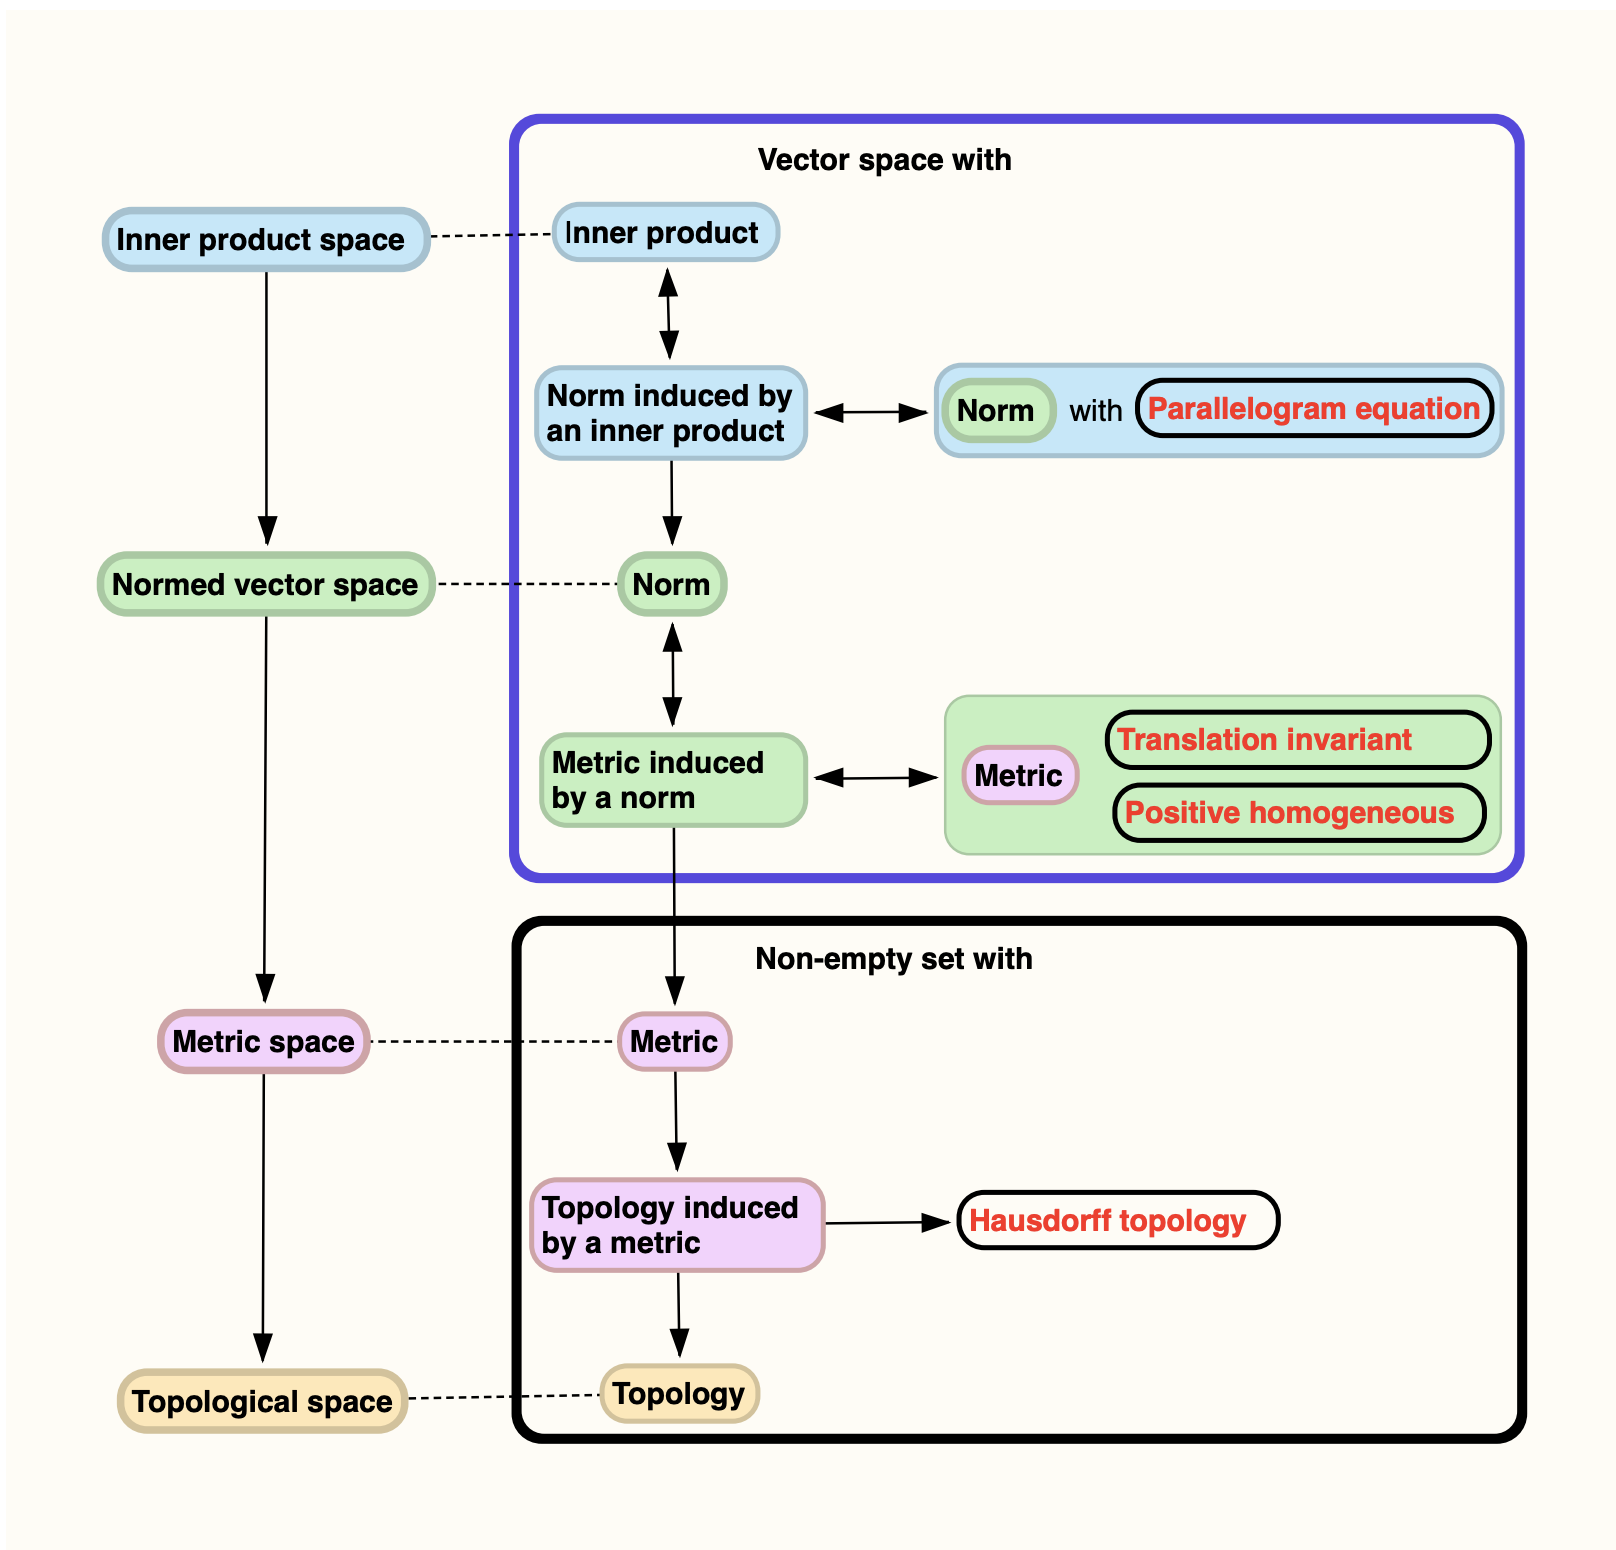
\includegraphics[height=10cm, width=15cm]{Relationship}
\caption{Relationships between spaces.}
\end{figure}
\end{center}

\begin{center}
\begin{figure}
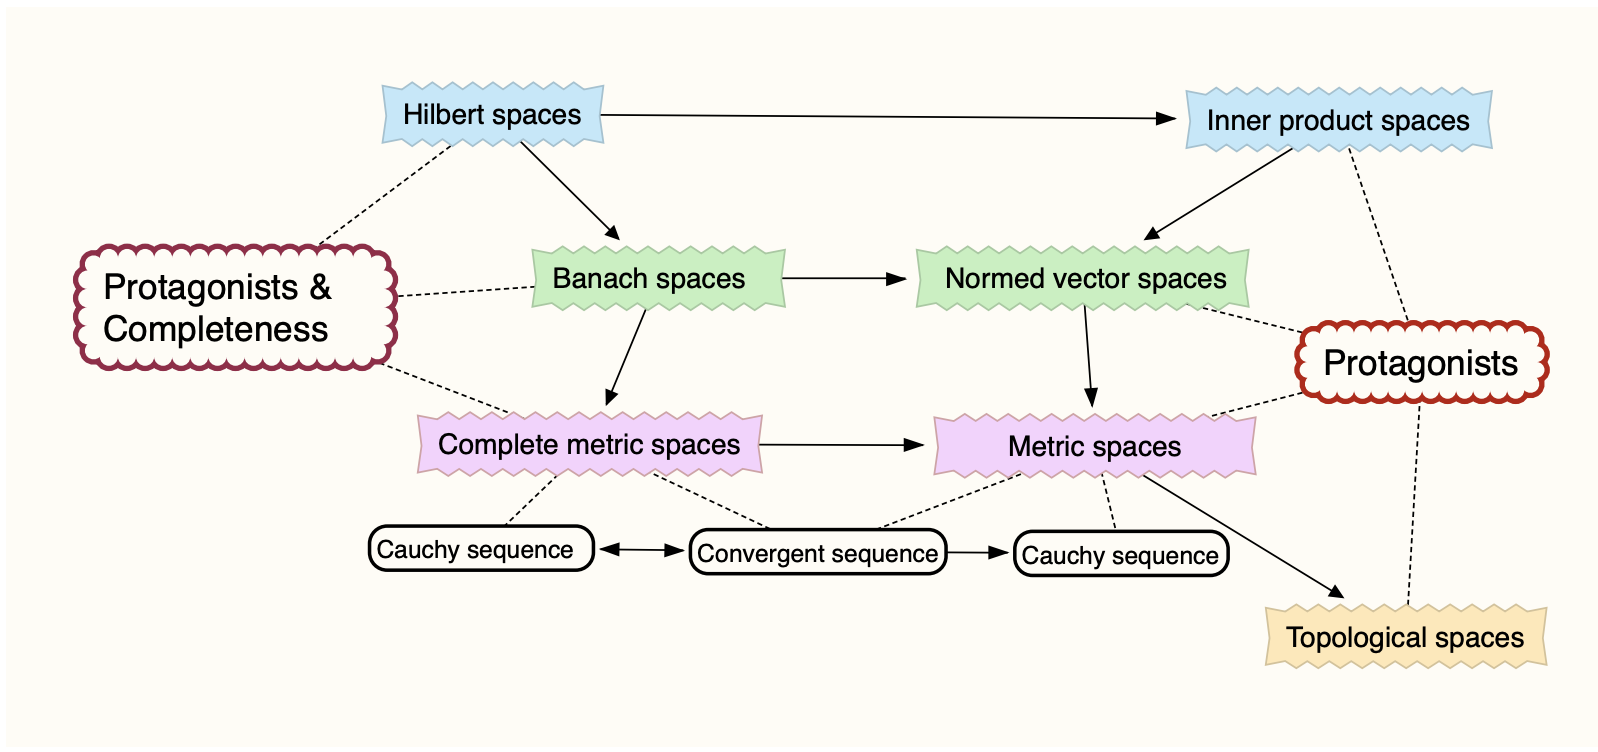
\includegraphics[height=9cm, width=15cm]{Completeness}
\caption{Relationships between complete spaces.}
\end{figure}
\end{center}

\lecture{2}{Vector Spaces and Inner Product Spaces}
\section{Vector Spaces}
\subsection{Vector Spaces}


\begin{definition}(Abelian Group). An abelian group is a set A together with an operation $\circ$ that combines any two elements $a, b \in A$ to form another element $a \circ b$. The set A and operation $\circ$ must satisfy
\begin{enumerate}
    \item Closure;
    \item Associativity;
    \item Identity element;
    \item Inverse element;
    \item Commutativity.
\end{enumerate}
\end{definition}

\begin{definition}(Vector Space). Let $(V, +)$ be an Abelian group, together with a scalar multiplication operation $\circ$, associating to each pair $(\alpha, v)$ in $\mathbb{K} \times V$ a vector $\alpha v$ in V. If the pair satisfies associativity, identity element and distributivity for all $\alpha, \beta \in \mathbb{K}$ and all vector $v, w \in V$, then V is called a vector space over $\mathbb{K}$.
\end{definition}

\begin{definition}We define $C([a,b];\mathbb{K})$ to be the space of all $\mathbb{K}$-valued continuous functions on [a,b].
\end{definition}

\begin{theorem}(Extreme Value Theorem). Every function in $C([a,b])$ that is bounded, attains its maximum as well as its minimum.
\end{theorem}

\begin{definition}(Bounded functions). We define $B([a,b];\mathbb{K})$ as the space of bounded functions on [a,b].
\end{definition}

\begin{definition}(p-summable sequence)We denote $\ell_p$ the set of all p-summable sequences in $\mathbb{K}$. A sequence $\{x_j\}_{j \geq 1} \in \mathbb{K}$ belongs to $\ell_p$ if and only if
$$
\sum_{j=1}^{\infty}|x_j|^p < \infty.
$$
\end{definition}

\begin{definition}(Linear Transformation). A mapping $T: X \rightarrow Y$ between vector spaces X and Y (over the same field $\mathbb{K}$) is called linear if for all $\alpha_1, \alpha_2 \in \mathbb{K}$ and every $x_1, x_2 \in X$, we have
$$
T(\alpha_1x_1 + \alpha_2x_2) = \alpha_1T(x_1) + \alpha_2T(x_2).
$$
When $Y = \mathbb{K}$, a linear transformation $T: X \rightarrow \mathbb{K}$ is called a $\textbf{linear functional}$ on X.
\end{definition}

\section{Inner Product Spaces}
\subsection{Inner Product Spaces}

The inner product on a vector space allows us to introduce the idea of the length and angle
 between vectors. 

\begin{definition}(Law of cosines). If the sides of a triangle have lengths a, b, and c, denoting by $\phi$ the angle made by the sides of length a and b, we have
$$
c^2 = a^2 + b^2 -ab cos\phi.
$$
\end{definition}


\begin{definition}(Triangle Inequality). For 2 vectors u and v, we have
$$
||u + v|| \leq ||u|| + ||v||.
$$
\end{definition}


\begin{definition}(Inner Product). Let $x = (x_1, x_2, ..., x_n)$ and $y = (y_1, y_2, ..., y_n)$ be in $\mathbb{K}^n$. The inner product on a vector space is a mapping which associates to each ordered pair of vectors, a scalar. We define it as
$$
\langle x, y \rangle = \sum_{j=1}^nx_j\bar{y}_j.
$$

This mapping $\langle . , . \rangle$ satisfies 
\begin{enumerate}
\item Positive definiteness;
\item Conjugate symmetry;
\item Linearity in the first argument.
\end{enumerate}
\end{definition}


\begin{definition}(Inner Product Space). Let V be a vector space and $\langle ., . \rangle$ be an inner product on V. Then $(V, \langle ., . \rangle)$ is known as an inner product space.
\end{definition}

\lecture{3}{Normed Vector Spaces}
\section{Normed Vector Spaces}
\section{Normed Vector Spaces}
\subsection{Normed Vector Spaces}
A normed vector space is a vector space in which a length (norm) can be assigned to each vector.


\begin{definition}(Norm). Let $||.||: V \rightarrow \mathbb{R}$. If $||.||$ satisfies the 3 properties of

\begin{enumerate}
\item Positive definiteness;
\item Positive homogeneity;
\item Triangle inequality;
\end{enumerate}
then $||.||$ is known as a norm. 
\end{definition}

\begin{definition}(Normed Vector Space). A normed vector space is a pair of a vector space V and a norm $||.||$.
\end{definition}

\begin{definition}(Norm induced by an inner product). We define a norm induced by an inner product as
$$
||x|| = \sqrt{\langle ., . \rangle}
$$
for every $x \in V$.
\end{definition}


\begin{definition}(Cauchy-Schwarz Inequality). For 2 vectors u and v, the norm induced by an inner product satisfies
$$
|\langle u, v \rangle| \leq ||u||\circ||v||.
$$
\end{definition}


\begin{definition}(Paralellogram Equation). For a triangle with sides u and v, the norm induced by an inner product satisfies
$$
||u + v||^2 + ||u - v||^2 = 2(||u||^2 + ||v||^2).
$$
\end{definition}

\begin{theorem}Every inner product space with the induced norm is a normed vector space.
\end{theorem}

\begin{definition}(Conjugate Exponent). 

Let $1 \leq p \leq \infty$. We denote p' as the conjugate exponent of p, that is
$$
\frac{1}{p} + \frac{1}{p'} = 1.
$$

For any $p \in (1,\infty)$, we have that
$$
p' = \frac{p}{p-1}.
$$
\end{definition}

\begin{lemma}(Young's Inequality).
For all $a, b \in [0, \infty)$, we have
$$
ab \leq \frac{1}{p}a^{p} + \frac{1}{q}b^{p'}.
$$
Moreover, equality holds if and only if $a^{p} = b^{p'}$.
\end{lemma}

\begin{lemma}(Hölder's inequality).

Let $n \geq 1$. If $x_j, y_j \geq 0$ for all $j = 1,...,n$, then
$$
\sum_{j=1}^{n}x_jy_j \leq \big(\sum_{j=1}^nx_j^{p}\big)\big(\sum_{j=1}^ny_j^{p'}\big)
$$
\end{lemma}

\begin{lemma}(Hölder's Inequality on C[a,b]).

Let $a, b \in \mathbb{R}$ with $a < b$. If $f, g \in C[a,b]$, then we have
$$
\int_a^b|f(x)g(x)|dx \leq (\int_a^{b}|f(x)|^{p}dx)(\int_a^b|g(x)|^{p'}dx).
$$

\end{lemma}

\begin{proposition}(Minkowski's Inequalities). Assume that $p \in [1, \infty)$.

\begin{enumerate}
\item Let $n \geq 1$. If $x_j, y_j \in \mathbb{K}$ for all $j = 1,2,...,n$, then we have
$$
\big(\sum_{j=1}|x_j + y_j|^p\big)^{\frac{1}{p}} \leq \big(\sum_{j=1}|x_j|^p\big)^{\frac{1}{p}} + \big(\sum_{j=1}|y_j|^p\big)^{\frac{1}{p}}.
$$
\item If $x_j, y_j \in \mathbb{K}$ for all $j \geq 1$ such that $\sum_{j=1}^{\infty}|x_j|^p < \infty$ and $\sum_{j=1}^{\infty}|y_j|^p < \infty$, then we have
$$
\big(\sum_{j=1}|x_j + y_j|^p\big)^{\frac{1}{p}} \leq \big(\sum_{j=1}|x_j|^p\big)^{\frac{1}{p}} + \big(\sum_{j=1}|y_j|^p\big)^{\frac{1}{p}}.
$$
\item Let $a,b \in \mathbb{R}$ with $a < b$. Assume that $f, g \in C[a,b]$. Then $(f + g) \in C[a,b]$ and 
$$
\big(\int_{a}^{b}|f(x) + g(x)|^{p}dx\big)^{\frac{1}{p}} \leq \big(\int_{a}^{b}|f(x)|^{p}dx\big)^{\frac{1}{p}} + \big(\int_{a}^{b}|g(x)|^{p}dx\big)^{\frac{1}{p}}.
$$
\end{enumerate}
\end{proposition}

\begin{corollary}Let $n \geq 1$ and $p \in (1, \infty)$. If $x_j, y_j \in \mathbb{K}$ for all $j = 1,...,n$, then
$$
\big|\sum_{j=1}^nx_jy_j\big| \leq \big(\sum_{j=1}^n|x_j|^p\big)^{\frac{1}{p}} + \big(\sum_{j=1}^n|y_j|^{p*}\big)^{\frac{1}{p*}}.
$$
\end{corollary}



\lecture{4}{Metric Spaces}
\section{Metric Spaces}
\section{Metric Spaces}
\subsection{Metrics}
\begin{definition}(Metric). A function d, assigning to every ordered pair of points x and y in a non-empty set X a real number d(x, y), is called a $\textbf{metric}$ (or distance) on X if it satisfies
\begin{enumerate}
    \item $d(x, y) \geq 0$ where d(x, y) = 0 if and only if x = y (Positive Definiteness) ;
    \item d(x, y) = d(y, x) (Symmetry);
    \item $d(x, z) \leq d(x, y) + d(y, z)$ (Triangle Inequality);
\end{enumerate}
for all points $x, y, z \in X$.
\end{definition}

\begin{definition}(Metric Space). A metric space is a $\textbf{non-empty}$ set with a metric.
\end{definition}

\begin{remark}Taking a non-empty subset Y of a metric space (X, d) with the original metric d will obtain you the $\textbf{metric subspace}$ of the original metric space (X, $d_Y$). 
\end{remark}

\begin{example}For all points $x = (x_1, x_2, ..., x_n)$ and $y = (y_1, y_2, ..., y_n)$ in $\mathbb{K}^n$, we define
\begin{enumerate}
\item $d_1(x, y) = \sum_{j=1}^n(x_j - y_j)$ (Taxicab Metric/Manhattan Metric);
\item $d_p(x, y) = \sum_{j=1}^n(|x_j - y_j|^p)^{\frac{1}{p}}$ (P-Metric);
\item $d_{\infty}(x, y) = \max_{1 \leq j \leq n}|x_j - y_j|$ (Supremum/Chebyshev Metric).
\end{enumerate}
\end{example}

\begin{remark}The power of the p-metric (1/p) is necessary for the p-metric to be a metric or else the triangle inequality can be violated.
\end{remark}

\lecture{5}{Metrics and The Topology of a Metric Space}
\section{Topology of a Metric Space}
\subsection{More Properties of Metrics}

Unlike norms which requires a vector space, metrics only require a set.

\begin{definition}(Discrete metric). The discrete metric $d_{dis}$ is defined by 
\[ d_{dis}(x,y) = \begin{cases}
        0 & x = y \\
        1 & x \neq y
    \end{cases}
\]
\end{definition}
\begin{lemma}Any set admits a metric by defining the $\textbf{discrete metric}$ on the set.
\end{lemma}

\begin{definition}(Metric induced by a norm). The metric induced by a norm on a vector space is defined as 
\[d(x,y) = ||x - y||\]
\end{definition}

\begin{theorem}Every normed vector space with its induced metric is a metric space.
\end{theorem}

We look at ways to determine whether is a metric is induced by a norm. We look at the properties of vector addition and scalar multiplication in vector spaces.
\begin{definition}(Translation-invariance). A metric d is called $\textbf{translation-invariant}$ if
\[d(x,y) = d(x+z, y+z)\] for every vectors x, y, and z.
\end{definition}
\begin{definition}(Positive-homogeneity). We say a metric d on a vector space is $\textbf{positive-homogeneous}$ if 
\[d(\alpha x, \alpha y) = |\alpha|d(x,y)\].
\end{definition}

\begin{theorem}A metric on a non-trivial vector space is induced by a norm if and only if the metric is translation-invariant $\textbf{and}$ positive-homogenous.
\end{theorem}

\begin{example}The discrete metric is not induced by a norm as it does not satisfy positive homogeneity.
\end{example}

\begin{lemma}Every translation-invariant and homogenous metric induces a norm by
$$
||x|| = d(x, 0).
$$
\end{lemma}

\section{Topology of a Metric Space}
\subsection{Definitions}
\begin{definition}(Open Ball). Let x be a point in a metric space (X, d) and $\epsilon > 0$. Then the set
$$
B_d(x;\epsilon) = \{y \in X: d(x, y) < \epsilon\}
$$
is known as the open $\epsilon$-ball about x.
\end{definition}

\begin{definition}(Open Set). A subset of X is called open if it contains an open ball about each of its points.
\end{definition}

\begin{definition}(Closed Ball). Let x be a point in a metric space (X, d) and $\epsilon > 0$. Then the set
$$
\bar{B}_d(x;\epsilon) = \{y \in X: d(x, y) \leq \epsilon\}
$$
is known as the closed $\epsilon$-ball about x.
\end{definition}

\begin{example}Let X be a set with the discrete metric $d_{dis}$. Then,
\[ B_{d_{dis}}(x;r)\begin{cases}
    \{x\} \quad r \leq 1 \\
    X \quad  r > 1
    \end{cases}
\]
\end{example}

\begin{theorem}Every open ball in a metric space is an open set.
\end{theorem}

\begin{definition}(Closed Set). A set in a metric space (X, d) is called closed if its complement in X is open.
\end{definition}

\begin{theorem}Every closed ball is a closed set in X.
\end{theorem}

\begin{theorem}For every metric space (X, d), each of the following is an open set.
\begin{enumerate}
    \item The empty set;
    \item The set X;
    \item $\textbf{Arbitrary}$ unions of open sets;
    \item $\textbf{Finite intersections}$ of open sets.
\end{enumerate}
\end{theorem}

\begin{theorem}(Metric Topology). The collection of all open sets in a metric space is called the topology induced by the metric or the $\textbf{metric topology}$.
\end{theorem}

\begin{remark}Note that a metric induces the idea of open balls, which induces the idea of open sets, which then induces a topology.
\end{remark}


\begin{theorem}A set in a metric space is open if and only if it can be written as a union of open balls.
\end{theorem}



\lecture{6}{Topology of Metric Spaces and Topologically Equivalent Metrics}
\section{Topology of a Metric Space}
\subsection{Topology of Metric Spaces}


\begin{definition}(Topology). A topology on a set X is a collection $\mathcal{T}$ of subsets of X such that\
\begin{enumerate}
\item Both the empy set and X are elements of $\mathcal{T}$;
\item Any union of elements of $\mathcal{T}$ is an element of $\mathcal{T}$;
\item Any intersection of finitely many elements of $\mathcal{T}$ is an element of $\mathcal{T}$.
\end{enumerate}
The members of $\mathcal{T}$ are called open sets.
\end{definition}
\begin{definition}(Topological Space). If $\mathcal{T}$ is a topology on X, then the pair (X, $\mathcal{T}$) is called a topological space.
\end{definition}

\begin{example} Example of arbitrary intersection of open sets is $(-1/n,1)$ which gives us the closed set [0,1) as $n \rightarrow \infty$.
\end{example}

\begin{definition}($\mathcal{T}$-open). Let (X, $\mathcal{T}$) be a topological space. Members of the topology $\mathcal{T}$ are called open relative to $\mathcal{T}$ or simply $\mathcal{T}$-open.
\end{definition}

\begin{definition}(Base of a topology). The base (or basis) $\textbf{B}$ for a topological space X with topology $\tau$ is a collection of open sets in X such that every open set X can be written as a union of elements of $\textbf{B}$.
\end{definition}

\begin{example} The family of all open balls in a metric space forms a base for the metric topology. Every open set can be expressed as the union of open balls.
\end{example}

\begin{theorem}A set in a metric space is open if and only if it is a union of open balls.
\end{theorem}

\begin{definition}(Open set in a topology). Let $(X, \tau)$ be a topological space. A set $A \subseteq X$ is open if for every point $a \in A$, there exists a neighbourhood U of x such that $x \in U \subseteq A$. 
\end{definition}

\subsection{Topologically Equivalent Metrics}
\begin{definition}(Topological Equivalence). Two metrics on the same set are $\textbf{topologically equivalent}$ if they induce the same topology. Equivalently, two metrics are topologically equivalent if the open sets in one metric topology coincides with the open sets in the other metric topology.
\end{definition}

\begin{lemma}(Nesting condition). Let there be two metrics on the same set X. Every open ball about any point in the set with respect to one metric contains an open ball about the same point in the other metric. \\Symbolically, let $d$ and $\rho$ be metrics on the same set X. The two metrics are topologically equivalent if and only if $\text{for every } x \in X \text{ and every } r > 0, \text{ there exists r', r''} > 0 \text{ such that}$
$$
\begin{cases}
B_{\rho}(x,r') \subseteq B_d(x,r) \\
B_{d}(x,r'') \subseteq B_{\rho}(x,r).
\end{cases}
$$
\end{lemma}

\begin{lemma}Two metrics on the same set are topologically equivalent if and only if the nesting condition holds.
\end{lemma}

\begin{example}Every metric space is homeomorphic to a bounded metric space. That is, for a metric space (X, d), it is homeomorphic to the metric space (X, d') where $d(x,y)' = min{1,d(x,y)}$.
\end{example}

\begin{definition}(Strongly equivalent). Two metrics d and $\rho$ on the same set X are called $\textbf{strongly equivalent}$ if there exists a $c > 0$ such that
$$
\frac{\rho(x,y)}{c} \leq d(x,y) \leq c\rho(x,y)
$$
for all $x, y \in X$.
\end{definition}

\begin{lemma}A sufficient condition for two metrics d and $\rho$ on the same set X to be $\textbf{topologically equivalent}$ if for all $x \in X$, there exists a $c_{x}$ such that 
$$
\frac{\rho(x,y)}{c_{x}} \leq d(x,y) \leq c_{x}\rho(x,y)
$$
for all $x, y \in X$.
\end{lemma}

\begin{remark}Strong equivalence implies the above lemma which implies topological equivalence.
\end{remark}

\begin{corollary}All p-metrics on $\mathbb{K}^n$ are strongly equivalent, where $1 \leq p \leq \infty$.
\end{corollary}

\lecture{7}{Topological Spaces}
\section{Topology of a Metric Space}
\subsection{Examples of topological spaces}

Many topologies can be placed on the same set X.

\begin{definition}(Indiscrete Topology). Let (X, $\mathcal{T}$) be a topological space. The indiscrete topology is such that only the empty set and set X is $\mathcal{T}$-open.
\end{definition}

\begin{definition}(Discrete Topology). Let (X, $\mathcal{T}$) be a topological space. The discrete topology is such that every subset of X is $\mathcal{T}$-open. Equivalently, it is the power set $\mathcal{P}$(X) of X.
\end{definition}

\begin{definition}(Cofinite Topology). Let (X, $\mathcal{T}$) be a topological space. The cofinite topology on X is the collection of all subsets of X with finite complements, together with the empty set.
\end{definition}

\subsection{Topological Spaces}

\begin{definition}(Isolated point of a subset). Let $(X, \mathcal{T})$ be a topological space. Let $H \subseteq X$. Then $x \in H$ is an isolated point of H if there exists an open set $\Omega \in \mathcal{T}$ such that 
$$
\{x\} = H \cap \Omega.
$$
In other words, there exists an open set of X that contains no other points of H other than x.
\end{definition}

\begin{definition}(Isolated point of a space). Let $(X, \mathcal{T})$ be a topological space. A point $x \in X$ is an isolated point if there exists an open set $\Omega \in \mathcal{T}$ such that 
$$
\Omega = \{x\}.
$$
\end{definition}

\begin{remark}A point x in a topological space is isolated if $\{x\}$ is open.
\end{remark}

\begin{remark} If $x \in X$ is an isolated point, then there exists a neighbourhood of x which does not contain any other point of X. In terms of metric spaces, there exists an open ball around the point containing only the point, hence the singleton set is open.
\end{remark}


\begin{theorem}A topological space is discrete if and only if each of its points is isolated.
\end{theorem}

\begin{proof}(Sketch). Every set $U \subseteq X$ is open as $U = \cup_{x \in U}\{x\}$ is the union of open sets which gives us an open set.
\end{proof}

\begin{lemma} Let $(X, \tau)$ be a discrete topological space. Then every open set is a clopen set.
\end{lemma}
\begin{proof} By definition, we have that $A \in \tau$ for every subset $A \subseteq X$. By definition of the topology, $A^c \in \tau$ as well. Hence, A is also closed.
\end{proof}

\begin{lemma} Every finite metric space is a discrete space.
\end{lemma}

\begin{lemma}The co-finite topology coincides with the discrete topology on a finite set.
\end{lemma}

\subsection{Metrization of topological spaces}

\begin{definition}(Metrizable Space). A topological space is called metrizable if its topology can be induced by a metric.
\end{definition}

\begin{remark} A metrizable space is a topological space that is $\textbf{homeomorphic}$ to a metric space. 
\end{remark}

\begin{definition}(Neighbourhood of a point). Let (X, $\mathcal{T}$) be a topological space and x is a $\textbf{point}$ in X. A neighbourhood of x is a subset $V \subset X$ that includes an $\textbf{open set}$ U containing x,
$$
x \in U \subseteq V.
$$
This is equivalent to $x \in X$ being in the interior of V.
\end{definition}

\begin{definition}(Hausdorff Property). Let (X, $\mathcal{T}$) be a topological space. The topological space satisfies the Hausdorff property if for every $x, y \in X$ such that $x \neq y$, there exists a neighbourhood U of x and a neighbourhood V of y such that
$$
U \cap V = \emptyset.
$$
\end{definition}

\begin{definition}(Hausdorff Space/$T_2$ space). A topological space (X, $\mathcal{T}$) satisfying the Hausdorff property is known as a Hausdorff space.
\end{definition}

\begin{theorem}Every metric space is a Hausdorff space.
\end{theorem}

\begin{theorem}($T_2$ axiom). A necessary condition for a topology to be metrizable is for the topological space to be a Hausdorff space.
\end{theorem}

\begin{lemma}Every singleton is a closed set in a Hausdorff space.
\end{lemma}

\begin{lemma}Any set endowed with the indiscrete topology is not Hausdorff.
\end{lemma}

\begin{lemma}An infinite topological space with the cofinite topology is not Hausdorff.
\end{lemma}

\subsection{Comparing Topologies}
\begin{definition}(Comparable topologies). Let X be a set and $\tau_1$ and $\tau_2$ be two topologies defined on X. If either $\tau_1 \subseteq \tau_2$ or $\tau_1 \supseteq \tau_2$, then $\tau_1$ and $\tau_2$ are said to be $\textbf{comparable}$. If $\tau_1 \subseteq \tau_2$, then $\tau_2$ is said to be the $\textbf{finer/stronger topology}$ and $\tau_1$ is said to be the $\textbf{coarser/weaker topology}$.
\end{definition}

\begin{remark} Two topologies on the same set need not be comparable.
\end{remark}

\begin{remark} In general, the union of two topologies is not necessarily a topology.
\end{remark}

\begin{remark}The indiscrete topology is the coarsest topology and the discrete topology is the finest topology. The intersection of topologies is the finest topology in all topologies.
\end{remark}


\subsection{Relative Topology}
\begin{definition}(Relatively Open). Let (X,d) be a metric space. Let $Y \subseteq X$ be a subset and we obtain the metric subspace $(Y,d_Y)$. A subset G of Y is called relatively open in Y if G is open in (Y, $d_Y$).
\end{definition}

\begin{remark} A set that is open in the metric subspace $(Y,d_Y)$ need not be open in the metric space $(X,d)$.
\end{remark}


\begin{definition}(Relative Topology/Topological Subspace). Let (X, $\mathcal{T}$) be a topological space. Let $Y \subset X$ be a non-empty subset of X. Then the $\textbf{relative topology}$ is defined as
$$
\mathcal{T}_Y = \{\Omega \cap Y: \Omega \in \mathcal{T}\}.
$$
\end{definition}

\begin{lemma}(Characterisation of open sets in relative topology). Let Y be a metric subspace of $(X,d)$. A subset of $A \subseteq Y$ is relatively open in Y if and only if $A = Y \cap \Omega$ for an open set $\Omega$ in $(X,d)$.
\end{lemma}

\begin{corollary}Let Y be a metric subspace of $(X,d)$. A subset of $A \subseteq Y$ is closed (in X) if there exists a closed set U in X such that $A = U \cap Y$.
\end{corollary}

\lecture{8}{Convergent Sequences and Equivalent Formulations of a Topology}
\section{Topology of a Metric Space}
\subsection{Convergent Sequences}

\begin{definition}(Sequence). A sequence $\{x_n\}_{n \geq 1}$ in a set X is a $\textbf{function}$ from the set of positive integers to X.
\end{definition}

\begin{definition}(Lies eventually). A sequence converges to x if for every open set U such that $x \in U$, there exists $N_U \in \mathbb{N}$ such that $x_n \in U$ for all $n \geq N_u$. A sequence is said to lies eventually if all but $\textbf{finitely}$ many terms belong to U.
\end{definition}

\begin{definition}(Convergence). A sequence $\{x_n\}_{n \geq 1}$ in a topological space X converges to a point x in X if the sequence lies eventually in every open set containing x, which is called the limit of $\{x_n\}$.
\end{definition}

\begin{definition}(Eventually constant). Let $(X, d)$ be a metric space. A sequence is eventually constant if there exists a $N \in \mathbb{N}$ such that for all $n \geq N$, $x_n = c$ for some $c \in X$.
\end{definition}

\begin{example} A sequence in X with the discrete topology converges to a point x in X if and only if the sequence is eventually constant.
\end{example}

\begin{example} A sequence in the same set X with the indiscrete topology converges to every point in X. If X has more than one point, then the limits of the sequences are not unique.
\end{example}

\begin{remark}Different topologies placed on a given set can cause the convergent sequences to differ and the limits may be different too as seen from the above examples.
\end{remark}

\begin{proposition}(Uniqueness of limits in Hausdorff spaces). Every convergent sequence in a Hausdorff space has a unique limit.
\end{proposition}

\begin{corollary}Every convergent sequence in a metric space has an unique limit.
\end{corollary}

\begin{lemma} Two metrics are topologically equivalent if and only if they have the same convergent sequences.
\end{lemma}

\begin{lemma}A sequence $\{x_n\}_{n \geq 1}$ converges to x in a metric space (X, d) if and only if the sequence of distances $\{d(x_n,x)\}_{n \geq 1}$ converges to 0 as $n \rightarrow \infty$.
\end{lemma}

\subsection{Equivalent Formulations of a Topology}
\begin{definition}(Closed Sets Axioms). A topological space is a set X together with a collection $\mathcal{A}$ of subsets of X, the members of which are called closed sets such that $\mathcal{A}$ contains $\emptyset$, X and is closed under both arbitrary intersections and finite unions.
\end{definition}

\begin{definition}(Closure). The closure $\bar{A}$ of a set A is the smallest closed set that contains A.
\end{definition}

\begin{definition}(Interior). The interior int(U) of a set U is the largest open set that is contained within U.
\end{definition}

\begin{lemma}A set is closed if and only if it is equal to its closure.
\end{lemma}

\begin{lemma}A set is open if and only if it is equal to its interior.
\end{lemma}

\begin{definition} (Interior, Closure and Boundary). Let U and A be subsets of a topological
space X. 
\begin{enumerate}
\item The interior of U, denoted by int(U), is the union of all open sets contained in U.
\item The closure of A, denoted by $\bar{A}$, is the intersection of all closed sets that contain A. 
\item The boundary of A, denoted by $\partial A$, is the closure of A without the interior of A, that is $\partial A \coloneqq \bar{A} - int (A)$.
\end{enumerate}
\end{definition}

\begin{definition}(Kuratowski's Closure Axioms). A topological space is a pair consiting of a set X and a function (closure) from $\mathcal{P}(X)$ to itself satisfying for every subsets A and B of X with the following axioms:
\begin{enumerate}
    \item The closure of the empty set is the empty set;
    \item The set A is a subset of its closure;
    \item The closure of the closure of A is the closure of A;
    \item The closure of the union $A \cup B$ is the union of the closure of A and the closure of B.
\end{enumerate}
\end{definition}

\begin{definition}(Neighbourhood of a point). A subset of a topological space is called a neighbourhood of a point x if it contains an open set containing x.
\end{definition}

\begin{definition}(Neighbourhood Axioms). A topological space consists of a set X together with a family $\mathcal{U} = \{\mathcal{U}_x\}_{x \in X}$ of sets $\mathcal{U}_x$ of subsets of X, called neighbourhoods of x such that
\begin{enumerate}
\item Every neighbourhood of x contains x and X is a neighbourhood of each of its points;
\item Every subset of X that contains a neighbourhood of x is itself a neighbourhood of x;
\item The intersection of any two neighbourhoods of x yields again a neighbourhood of x;
\item Within every neighbourhood of x lies a neighbourhood of x that is a neighbourhood of each of its points.
\end{enumerate}
\end{definition}

\lecture{9}{Closure of a set and Limit Points}
\section{Topology of a Metric Space}
\subsection{Closure of a set and Limit Points}
\begin{proposition} Let Y be a subspace of a topological space X. If $A \subset Y$, then the closure of A in Y is
$$
Y \cap \bar{A}.
$$
\end{proposition}


\begin{remark}The closure of a set refers to the smallest closed set with respect to the whole space that covers the set. The above formulation refers to the smallest closed set in the space Y that covers our set of interest A. Note that the notation $\bar{A}$ refers to the closure with respect to the whole space X. We need to be careful to distinguish between closed sets in Y and closed sets in X.
\end{remark}

\begin{definition}(Intersection of sets). Two sets intersect if their intersection is not empty.
\end{definition}

\begin{definition}(Limit point/Accumulation points/Cluster point). Let $A \subset X$ in $(X, \tau)$. A point $x \in X$ is called a limit point of A if every neighbourhood of x intersects A\textbackslash $ \{x\}$.
\end{definition}

\begin{remark}Every neighbourhood of x in A contains another point from A. Hence, we can approximate x with points in A. This generalises what a limit is.
\end{remark}

\begin{remark}Note that in a metric space (X, d), a point $x \in A \subseteq X$ is a limit point of A if for every ball $B_d(x, \epsilon)$, there exists an $a \in A$ such that $a \in B_d(x, \epsilon)$ for all $\epsilon > 0$.
\end{remark}

\begin{definition}(Derived set). The derived set of A, written as $A'$, is the set of all limit points of A.
\end{definition}

\begin{theorem}(Characterization of closure). Let A be a subset of a topological space $(X, \tau)$.
\begin{enumerate}
    \item A point $x \in X$ belongs to $\bar{A}$ if and only if every neighbourhood of x intersects A.
    \item $\bar{A} = A \cup A'$.
\end{enumerate}
\end{theorem}

\begin{corollary}A set in a topological space is closed if and only if it contains all its limit points.
\end{corollary}

\begin{definition}(Dense sets for topological spaces). A subset A of a topological space X is called $\textbf{dense}$ if $\bar{A} = X$.
\end{definition}

\begin{remark}This means that every point in X is either in the set A or a limit point of A.
\end{remark}

\begin{remark}For a metric space (X, d), a set $A \subseteq X$ is dense in X if for every $x \in X$ and for all $\epsilon > 0$, there exist an element $a \in A$ such that $a \in B_d(x;\epsilon)$.
\end{remark}

\begin{theorem}Let $(X, \tau)$ be a topological space and let $A \subseteq X$. Then A is dense in X if and only if for every $U \in \tau$\textbackslash$\{\emptyset\}$, we have that $A \cap U \neq \emptyset$.
\end{theorem}

\begin{example}(The set of rational numbers $\mathbb{Q}$ is dense in $\mathbb{R}$). The set set of rational numbers $\mathbb{Q} \subset \mathbb{R}$ is dense in the topological space $(\mathbb{R}, \tau)$ where $\tau$ is the topology of open intervals. Recall from Analysis that there is always a natural number in between two real numbers through the Archmidean property.
\end{example}

\begin{definition}(Countable set). A set is countable if there exists an injective map from it to the set $\mathbb{N}$ of natural numbers.
\end{definition}

\begin{definition}(Separable). A topological space is called separable if it admits a countable dense subset.
\end{definition}

\begin{lemma}Every singleton in a Hausdorff space is a closed set.
\end{lemma}

\begin{definition}($T_1$-space). A topological space in which every singleton is a closed set is called a $T_1$-space. In other words, for every pair of points in X, there exists disjoint neighbourhoods of the points.
\end{definition}

\begin{theorem}(Characterisation of limit points in $T_1$-space). Let A be a subset of a $T_1$-space X. A point $x \in X$ is a limit point of A if and only if every neighbourhood of x contains infinitely many points of A.
\end{theorem}

\begin{theorem}For every subset A of a $T_1$-space, the derived set $A'$ is closed.
\end{theorem}

\begin{definition}(Local base). Let $(X, \tau)$ be a topological space and let $x \in X$. A local base of the element x is a collection of open neighbourhoods of x, $\mathcal{B}_x$, such that for every $U \in \tau$ where $x \in U$, there exists a $B \in \mathcal{B}_x$ such that $\mathcal{B}_x \in U$.

In other words, a local base at a point x in a topological space is a collection $\mathcal{B}_x$ of open neighbourhoods of x such that every neighbourhood of x contains a member of $\mathcal{B}_x$.
\end{definition}

\begin{definition}(First-countable).
A topological space is called $\textbf{first-countable}$ if at each of its points, there exists a countable local base.
\end{definition}

We look at a few basic theorems relating local bases and basis of the topology.
\begin{theorem}Let $(X, \tau)$ be a topological space and let $\mathcal{B}$ be a basis of $\tau$. Then for each $x \in X$, we have that $\mathcal{B}_x = \{B \in \mathcal{B}: x \in B \}$ is a local basis of x.
\end{theorem}

\begin{theorem}Let $(X, \tau)$ be a topological space. Let $\{\mathcal{B}_x\}_{x \in X}$ be a collection of local bases for each $x \in X$. Then $\mathcal{B} = \cup_{x \in X}\mathcal{B}_x$ is a basis for $\tau$.
\end{theorem}


\begin{theorem}Let A be a subset of a $\textbf{first-countable space}$ X.
\begin{enumerate}
\item A point $x \in X$ is a limit point of A if and only if x is the limit of a sequence of points in A \textbackslash $\{x\}$.
\item A point $x \in X$ belongs to the closure of A if and only if it is the limit of a sequence in A.
\end{enumerate}
\end{theorem}

\begin{definition}(Sequentially open sets/Sequentially closed sets). Let X be a topological space. A subset $U \subset X$ is called sequentially open if for every sequence in X that converges to a point in U, lies eventually in U. We say that a subset $F \subset X$ is sequentially closed if whenever a sequence in F converges in X, then its limit belongs to F.
\end{definition}

\begin{theorem}In any topological space, every open set is sequentially open and every closed set is sequentially closed.
\end{theorem}

\begin{theorem}In a $\textbf{first-countable space}$, a set is open if and only if it is sequentially open and, similarly, a set is closed if and only if it is sequentially closed.
\end{theorem}

\begin{remark}In a topological space, an open set is a sequentially open set. In a Hausdorff space, a set is open if and only if it is sequentially open.
\end{remark}

\begin{remark}In an arbitrary topological space, a sequentially closed set $\textbf{does not}$ imply a closed set. However, it does hold in a metric space as it is a first countable space.
\end{remark}

\lecture{10}{Cauchy Sequence and Completeness of Metric Spaces}
\section{Topology of a Metric Space}
\subsection{Cauchy Sequence and Completeness of Metric Spaces}

\begin{definition}(Cauchy Sequence). A sequence $\{x_n\}_{n \geq 1}$ in a metric space (X, d) is called a Cauchy sequence if for every $\epsilon > 0$, there exists $n_{\epsilon} \geq 1$ such that $d(x_m, x_n) < \epsilon$ for all $m, n \geq n_{\epsilon}$.
\end{definition}

\begin{definition}(Diameter of a set). Given a metric space (X, d) and a non-empty subset A of X, the diameter of A, denoted by diam A, is defined by $$diam A \coloneqq \sup\{d(x,y): x,y \in A\}. $$
\end{definition}

\begin{definition}(Bounded set). We say that $A \subset X$ is bounded if diam A $< \infty$.
\end{definition}

\begin{lemma} Let (X, d) be a metric space and $A \subseteq X$. The set A is bounded if and only if for every $x \in A$, there exists $r > 0$ so that $A \subseteq B_d(x,r)$.
\end{lemma}

\begin{lemma} Let (X, d) be a metric space and $A \subseteq X$. Every finite set A is bounded.
\end{lemma}

\begin{lemma} Every Cauchy sequence in $(X, d)$ is a bounded set.
\end{lemma}

\begin{lemma} Every metric space is a Hausdorff space so that each convergent sequence in a metric space has a unique limit.
\end{lemma}

\begin{definition}(Complete Metric Space). A metric space is called complete if every of its Cauchy sequence converges to a point in the space.
\end{definition}

\begin{lemma}Let (X, d) be a metric space.
\begin{enumerate}
\item Any convergent sequence is a Cauchy sequence.
\item If a Cauchy sequence contains a convergent subsequence, then the whole sequence converges to the same limit.
\end{enumerate}
\end{lemma}

\begin{corollary}A metric space is complete if and only if every Cauchy sequence has a convergent subsequence.
\end{corollary}


\begin{remark} Not every Cauchy sequence is convergent. A Cauchy sequence is convergent if it contains a convergent subsequence.
\end{remark}

\begin{proposition}Every Cauchy sequence in discrete space is eventually constant.
\end{proposition}

\begin{proof}(Sketch). Every Cauchy sequence in discrete space is eventually constant. Every eventually constant sequence is convergent.
\end{proof}

\subsection{Examples of Complete Metric Spaces}

We recall from Analysis the completeness of $\mathbb{K}^N$.

\begin{theorem}(Bolzano-Weierstrass theorem). Let $\{x_n\}_{n \geq 1}$ be a bounded sequence. Then, the sequence has a convergent subsequence.
\end{theorem}

\begin{theorem}(Completeness of $\mathbb{K}^N$). Let $\{x_n\}_{n \geq 1}$ be a Cauchy sequence in $\mathbb{K}^N$. Then,
\begin{enumerate}
\item Every Cauchy sequence is bounded in $\mathbb{K}^N$;
\item Every Cauchy sequence contains a convergent subsequence by the Bolzano-Weierstrass theorem.
\item Every Cauchy sequence that contains a convergent subsequence converges to the limit of its convergent subsequence.
\end{enumerate}
Hence, every Cauchy sequence in $\mathbb{K}^N$ converges in $\mathbb{K}^N$.
\end{theorem}

\begin{theorem}(Completeness of $(C([a,b],\mathbb{K}),d_{\infty})$). Let $C[a,b]$ be the space of all $\mathbb{K}$-valued continuous functions on [a,b]. Let $d_{\infty}(f,g) = \sup_{x \in [a,b]}|f(x) - g(x)|$ be the supremum norm.\\ $(C([a,b],\mathbb{K}),d_{\infty})$ is a Banach space.
\end{theorem}

\begin{theorem}(Completeness of $(B([a,b],\mathbb{K}),d_{\infty})$). Let $B[a,b]$ be the space of all $\mathbb{K}$-valued $\textbf{bounded}$ functions on [a,b]. Let $d_{\infty}(f,g) = \sup_{x \in [a,b]}|f(x) - g(x)|$ be the supremum norm.\\ Then $(B([a,b],\mathbb{K}),d_{\infty})$ is a Banach space.
\end{theorem}

\begin{theorem}(Completeness of $\ell_p$). Let $\ell_p = \{x = \{x_j\}_{j \geq 1}: \sum_{j=1}^{\infty}|x_j|^p < \infty\}$ for $1 \leq p < \infty$. Define $d(x,y) = \bigg( \sum_{j=1}^{\infty}|x_j-y_j|^p \bigg)^{1/p}.$\\ Then $(\ell_p, d)$ is a Banach space.
\end{theorem}

\begin{theorem}(Completeness of $\ell_{\infty}$). Let $\ell_{\infty} = \{x = \{x_j\}_{j \geq 1}: \sup_{i \in \mathbb{N}}|x_i| < \infty\}$. Define $d_{\infty}(x,y) = \bigg( \sup_{i \in \mathbb{N}}|x_i - y_i| \bigg).$\\ Then $(\ell_{\infty}, d_{\infty})$ is a Banach space.
\end{theorem}


\begin{theorem} Let $(X, d)$ be a complete metric space. A subspace of a complete metric space is complete if and only if it is closed.
\end{theorem}
\begin{remark}If we have a space which we know is a subspace of a complete metric space, to show that it is complete, it suffices to show that the subspace is closed.
\end{remark}

\begin{theorem}(Completeness of c). Let c be the space of all convergent sequences in $\mathbb{K}$. Let $d_{\infty}(x,y) = \sup_{i \in \mathbb{N}}|x_i - y_i|$.\\ Then $(c, d_{\infty})$ is a Banach space.
\end{theorem}

\begin{theorem}(Completeness of $c_0$). Let $c_0$ be the space of all sequences in $\mathbb{K}$ that converges to 0. Let $d_{\infty}(x,y) = \sup_{i \in \mathbb{N}}|x_i - y_i|$.\\ Then $(c_0, d_{\infty})$ is a Banach space.
\end{theorem}

\subsection{Examples of Incomplete Metric Spaces}
\begin{theorem}Let $C[0,1]$ be the space of continuous functions on [0,1]. We define the p-norm as $\int_{0}^{1}|f(x)-g(x)dx$. The space C[0,1] with the p-norm is $\textbf{incomplete}$.
\end{theorem}

\begin{theorem}Let $c_{00}$ be the space of all sequences in $\mathbb{K}$ with at most finitely many non-zero terms. Then $c_00$ is an incomplete subspace of the Banach space $\ell_{\infty}$ as it is $\textbf{not}$ a closed subspace.
\end{theorem}

\lecture{11}{Cantor's Intersection Theorem}
\section{Topology of a Metric Space}
\subsection{Cantor's Intersection Theorem}

\begin{remark}Completeness is not topologically invariant. That is, if a metric space is complete and its topology induced is topologically equivalent to another metric space's topology, that does not mean that the other metric space is complete.
\end{remark}

\begin{lemma}We have the descending order of hierarchy for properties of a sequence.
\begin{enumerate}
\item Convergent sequence;
\item Cauchy sequence;
\item Bounded sequence.
\end{enumerate}
\end{lemma}

\begin{definition}(Nested sequence). Let (X, d) be a metric space. Then a sequence of $\{X_n\}$ of sets in X is said to be a nested sequence if $X_n \supseteq X_{n+1}$ for all n.
\end{definition}

The following is a characterization of a complete metric space.

\begin{theorem}(Cantor's Intersection Theorem). A metric space (X, d) is complete if and only if whenever a sequence $\{F_n\}_{n \geq 1}$ of non-empty subsets of X satisfies
\begin{enumerate}
\item $F_n$ is a closed set for all $n \geq 1$;
\item $F_1 \supseteq F_2 \supseteq ... \supseteq F_n \supseteq F_{n+1}$ for all $n \geq 1$;
\item diam $(F_n) \rightarrow 0$ as $n \rightarrow \infty$,
\end{enumerate}
then $\bigcap_{n=1}^{\infty}F_n = \{x\}$ is a $\textbf{single point}$ where x is a unique point common to all $F_n$.
\end{theorem}

\lecture{12}{Baire Category Theorem}
\section{Topology of a Metric Space}
\subsection{Baire Category Theorem}

\begin{definition}Let (X, d) be a metric space. We say that $A \subseteq X$ is dense in X if $\bar{A} = X$.
\end{definition}

\begin{lemma}Let $(X, \tau)$ be a topological space. Then let $\{D_1, ..., D_m\}$ be a sequence of open $\textbf{dense}$ sets in X. Then the $\textbf{finite}$ intersection
$$
\bigcap_{i=1}^mD_i
$$
is also an $\textbf{open}$ and dense set.
\end{lemma}


\begin{remark}In $\textbf{general}$, a countable intersection of open dense sets in a topological space is $\textbf{not}$ dense.
\end{remark}

\begin{definition}(Baire Space). A topological space is called a Baire space if every countable intersection of open dense sets in X is also dense in X.
\end{definition}

We look at the sufficient conditions for a topological space to be a Baire space.


\begin{theorem}(Baire Category Theorem). Every complete metric space is also a Baire space.
\end{theorem}

\begin{proposition}Every open subspace of a Baire space is also a Baire space.
\end{proposition}

\begin{definition}(Nowhere Dense). Let (X, d) be a metric space. A subset Y of X is called nowhere dense if $\bar{Y}$ has no interior points, that is, int($\bar{Y}$) = $\emptyset$. Alternatively, for every $U \in \tau$, where $\tau$ is the topology induced by the metric d, there exists a $A \subseteq U$ such that $\bar{A} \cap Y = \emptyset$.
\end{definition}

\begin{lemma}The subset Y of X is nowhere dense if and only if X \textbackslash $\bar{Y}$ is a dense open subset of X.
\end{lemma}

\begin{remark}A nowhere dense set can be thought of a dense that is so small that it has no open ball inside of it.
\end{remark}

\begin{theorem}Let $A \subseteq X$ be nowhere dense. Then for $B \subseteq A$, we have that B is nowhere dense.
\end{theorem}

\begin{theorem} Let (X, d) be a complete metric space. Let $\{E_n\}_{n \geq 1}$ be a sequence of nowhere dense subsets of X. Then $\bigcup_{n=1}^{\infty}E_n$ is nowhere dense in X.
\end{theorem}

\begin{remark}If we have a collection of sets that contain no open ball inside of them, then the union will not contain an open ball.
\end{remark}


\begin{corollary}The set $\mathbb{R}$ is uncountable.
\end{corollary}

\begin{definition}(First Category/Meagre). Let (X, d) be a metric space. A subset $Y \subseteq X$ is called of the first category if Y can be expressed as a countable union of nowhere dense sets. Otherwise, it is called of the second category.
\end{definition}

\begin{theorem}Let $(X, \tau)$ be a topological space. Let $\{A_i\}_{i \in I}$ be a collection of sets of the first category. Then $\bigcup_{i \in I}A_n$ is of the first category.
\end{theorem}


\begin{theorem}(Baire Category theorem). A complete metric space is of the second category.
\end{theorem}

\begin{remark}Let X be a complete metric space and we express it as the union of closed sets i.e. $X = \cup_{i=1}^{\infty}A_i$. By the Baire category theorem, at least one of these sets must contain an open ball.
\end{remark}

\begin{theorem}A subspace of a complete metric space is complete if and only if the subset is a closed set.
\end{theorem}

\begin{remark}Baire category theorem shows that every complete metric space is a Baire space. However, a Baire space need not be a metric space nor complete.
\end{remark}

\begin{proposition}Any open subspace of a Baire space is a Baire space.
\end{proposition}

\lecture{13}{Continuous Functions}
\section{Continuous Functions}
\section{Continuous Functions}
\subsection{Continuous Functions}

\begin{definition}(Global continuous function). Let $(X, \tau_X)$ and $(Y, \tau_Y)$ be topological spaces. A function $f: X \rightarrow Y$ is called continuous if whenever V is open in Y, we have that $f^{-1}[V]$ is open in X.
\end{definition}

\begin{proposition} A function $f: X \rightarrow Y$ is continuous if and only if for every closed set $B \subseteq Y$, $f^{-1}[B]$ is closed in X.
\end{proposition}

We look at different formulations of continuity.

\begin{proposition}Define the function between topological spaces $f: X \rightarrow Y$. The following are equivalent.
\begin{enumerate}
\item f is continuous.
\item $f(\bar{A}) \subseteq \overline{f(A)}$ for every $A \subseteq X$.
\item $\overline{f^{-1}[B]} \subseteq f^{-1}[\bar{B}]$ for every $B \subseteq Y$.
\item $f^{-1}[int(B)] \subseteq int(f^{-1}[B])$.
\end{enumerate}
\end{proposition}

\begin{definition}(Pointwise continuous). Let $(X, \tau_X)$ and $(Y, \tau_Y)$ be topological spaces. A function $f: X \rightarrow Y$ is continuous at a point $x \in X$ if for all open sets V in Y such that $f(x) \in V$, there exists an open set U in X such that $x \in U$ and $f(U) \subseteq V$. In otherwords, the preimage of any neighbourhood of f(x) is a neighbourhood of x.
\end{definition}

\begin{theorem}Let X and Y be topological spaces. A function $f: X \rightarrow Y$ is continuous if and only if f is continuous at every point of X.
\end{theorem}

\begin{theorem}Let $X, Y, Z$ be topological spaces. Let $f: X \rightarrow Y$ and $g: Y \rightarrow Z$ be continuous. Then $g \circ f: X \rightarrow Z$ is also continuous.
\end{theorem}

\begin{lemma} Let the function f map between the topological spaces $f: X \rightarrow Y$.
\begin{enumerate}
\item Every function f is continuous if X is the discrete topology;
\item Every function f is continuous if Y is the indiscrete topology.
\end{enumerate}
\end{lemma}

\subsection{Homeomorphisms}
\begin{definition}(Homeomorphism). Let X and Y be topological spaces. A function $f: X \rightarrow Y$ is called a homeomorphism if
\begin{enumerate}
\item f is bijective;
\item f is continuous;
\item $f^{-1}$ is continuous.
\end{enumerate}
\end{definition}

\begin{remark}$f: X \rightarrow Y$ is also a homeomorphism if f is bijective and U is open in X if and only if $f(U)$ is open in Y.
\end{remark}

\begin{lemma}A bijective continuous map is a homeomorphism if and only if it an open map if and only if it is a closed map.
\end{lemma}

\begin{definition}(Homeomorphic spaces). We say that X and Y are homeomorphic (topologically equivalent) if there exists a homeomorphism $f: X \rightarrow Y$.
\end{definition}

Homeomorphic spaces are topologically equivalent.

\begin{example}The space $[0,r)$ and $[0,\infty)$ is homeomorphic by the homeomorphism $f(t) = \frac{x}{1+t}$ for $t \in [0,r)$.
\end{example}

\begin{lemma}The following are homeomorphisms:
\begin{enumerate}
\item The identity map $\phi: X \rightarrow X$;
\item The inverse of a homeomorphism is also a homeomorphism;
\item The composition of homeomorphism is also a homeomorphism.
\end{enumerate}
\end{lemma}

\begin{theorem}Let $(X, \tau)$ be a topological space and (Y, d) be a metric space. A function $f: X \rightarrow Y$ is continuous at $x \in X$ if and only if for all $\epsilon > 0$, there exists a neighbourhood U of x such that $d(f(x), f(y)) < \epsilon$ for all $y \in U$.
\end{theorem}

\subsection{Topological Properties}
\begin{definition}(Topological property). A property of a topological space is called topological if it is preserved under homeomorphisms.
\end{definition}

\begin{proposition} The following are topological properties.
\begin{enumerate}
\item Discrete.
\item Separable.
\item Metrizable.
\item Finite/Countable/Uncountable.
\item Hausdorff Property.
\end{enumerate}
\end{proposition}

\begin{proposition}Let $f:X \rightarrow Y$ be a homeomorphism.
\begin{enumerate}
\item $f(\bar{A}) = \overline{f(A)}$.
\item f(int(A)) = int(f(A)).
\item $f(\partial A) = \partial f(\partial A)$.
\item If $x_n \rightarrow x$ in X, then $f(x_n) \rightarrow f(x)$ in Y.
\end{enumerate}
\end{proposition}

\lecture{14}{Finite product of metric spaces}
\section{Continuous Functions}

\subsection{Initial Topology}

Often, we start with a topology and ask if this function continuous. Now we are interested in the reverse. Starting with a function, what type of topology will make the function continuous.

\begin{definition}(Initial Topology). Let X and $Y_i$ be topological spaces where $i \in I$. The initial topology induced by $\{f_i\}_{i \in I}$ on X is the $\textbf{coarsest}$ topology on X that makes each map $f_i: X \rightarrow Y_i$ continuous.
\end{definition}

Starting off with a topology on each space $Y_i$, we require that the preimage of every open set on every topological space $Y_i$ is open in X. Hence, we construct a topology on X that satisfies this. We define a set to be open in X by selecting the preimage of every open set on every topological space. This gives us the coarsest topology and hence the inital topology.

\begin{remark}Note that as a last resort, letting X be a discrete space will ensure that every $\{f_i\}_{i \in I}$ is continuous.
\end{remark}

\subsection{Finite Product of topological spaces}

The product topology, is a special case of the initial topology with respect to the family of projection maps.

\begin{definition}(Product Topology/Tychonoff topology). Let $\{X_1,...,X_n\}$ be finite collection of topology sets with the resulting topological product being the set $\prod_{i=1}^nX_i$. The product topology is then defined to be 
$$
\mathcal{B} = \{\prod_{i=1}^nU_i: U_i \text{ is open in }X_i: \text{ for i } \in \{1,...,n\}\}.
$$
\end{definition}

\begin{theorem} The topological products $X \times Y$ and $Y \times X$ are homeomorphic to each other.
\end{theorem}

\begin{theorem}Let $\{X_1,...,X_n\}$ be finite collection of topology sets with the resulting topological product being the set $\prod_{i=1}^nX_i$. Define $p_j$ for j=1,...,n to be the projection maps such that $p_j: \prod_{i=1}^nX_i \rightarrow X_j$. Then 
\begin{enumerate}
\item Each $p_j$ is surjective, open, and continuous.
\item The initial topology on $\prod_{i=1}^nX_i$ is the product topology.
\end{enumerate}
\end{theorem}

\begin{theorem}
Let each $X_i$ for $i \in \{1,2,...,n\}$ hold property $\mathcal{P}$. Then property $\mathcal{P}$ also holds for $\prod_{i=1}^nX_i$. Property $\mathcal{P}$ include
\begin{enumerate}
\item First countable
\item Second countable
\item Separable
\item Hausdorff
\item Metrizable.
\end{enumerate}
\end{theorem}

\begin{theorem}Let $A_i \subseteq X_i$ for $i \in \{1,2,...,n\}$ be dense subsets. Then $\prod_{i=1}^nA_i$ is dense in $\prod_{i=1}^nX_i$.
\end{theorem}

\subsection{Finite product of metric spaces}

\begin{definition}(Finite product of metric spaces). Let $(X_1,d_1),...,(X_n,d_n)$ be metric spaces. Let the product set be $X = X_1 \times X_2 \times ... \times X_n$ which consists of all n-tuples $(x_1,...,x_n)$ where $x_k \in X_k$ for every k = 1,...,n. Define d to be the $\textbf{product metric}$ on this space. Then (X, d) is known as the finite product of metric spaces.
\end{definition}

\begin{definition}(Properties of product metric). The two properties we would want the metric d on the product set X to have are listed below:
\begin{enumerate}
\item A sequence $\{x^{(j)}\}_{j \geq 1} = (x_{1}^{(j)},...,x_{n}^{(j)})_{j \geq 1}$ converges to $x = (x_1,...,x_n)$ in (X,d) if and only if for each k=1,...,n, the sequence of component entries $\{x_{k}^{(j)}\}_{j \geq 1}$ converges to $x_k$ in $(X_k,d_k)$.
\item $d_k(x_k,y_k) \leq d(x,y)$ for all $x,y \in X$ for all $k=1,...,n.$
\end{enumerate}
\end{definition}

\begin{remark}Property (2) neither implies nor is implied by property (1). However, if property (2) holds, then whenever a sequence $\{x^{(j)}\}_{j \geq 1}$ converges to $x = (x_1,...,x_n)$ in (X,d), then each of the component sequences $\{x_{k}^{j}\}_{j \geq 1}$ converges to $x_k$ in $(X_k,d_k)$ for each k=1,...,n.
\end{remark}

\begin{theorem}Let $(X_1,d_1),...,(X_n,d_n)$ be complete metric spaces. Let d be a product metric on $X = X_1 \times ... \times X_n$ that satisfies property (1) and property (2). Then (X,d) is complete.
\end{theorem}

\begin{theorem}Suppose that d is a metric on $X = X_1 \times ... \times X_n$ which satisfies property (1). Define
$$
\mathcal{B} = \{\Omega \subseteq X: \text{ there exists an open set } U_k \in (X_k,d_k) \text{ for } 1 \leq k \leq n \text{ such that } \Omega = U_1 \times ... \times U_n\}.
$$
Then the open sets in (X,d) are the unions of sets in $\mathcal{B}$.
\end{theorem}

For any topological space Y, we can construct a continuous function from Y to the finite product of metric spaces.
\begin{theorem}Let $(X_k,d_k)$ be metric spaces for k=1,...,n. Let $X = X_1 \times ... \times X_n$ be endowed with a metric d which satisfies condition (1). Define the projection $\pi_k: X \rightarrow X_k$ by $\pi_k(x) = x_k$ where $x = (x_1,...,x_n) \in X$ for each k=1,...,n. 
\begin{enumerate}
\item Each $\pi_k: X \rightarrow X_k$ is continuous for all k=1,...,n.
\item Let Y be any topological space. Then a function $f:Y \rightarrow X$ is continuous if and only if $\pi_k \circ f: Y \rightarrow X_k$ is continuous for all k=1,...,n.
\end{enumerate}
\end{theorem}

\lecture{15}{Sequential continuity}
\section{Continuous Functions}
\subsection{Sequential continuity}
\subsection{Sequential Continuity}

Recall that any open set is sequentially open but $\textbf{not the converse for arbitrary topological spaces}$. However, in a first countable space, it holds both ways.

\begin{definition}(Sequentially continuous function). A function $f:X \rightarrow Y$ between topological spaces X and Y is called sequentially continuous if whenever $\{x_n\}$ converges to x in X, we have $\{f(x_n)\}$ converges to f(x) in Y.
\end{definition}

Sequential continuity is a weaker form of continuity.

\begin{theorem}(Relation between continuity and sequential continuity). Every continuous map between topological spaces is sequentially continuous. Conversely, every sequentially continuous map from a $\textbf{first-countable}$ space to a topological space is continuous.
\end{theorem}

\begin{remark}If we have a first-countable space, to show that the preimage of an open set is open, it suffices to show that the preimage is sequentially open, that is, every sequence that converges to a point in the set lies eventually in the set.
\end{remark}

It is much easier to show sequentially continuity of a function which we should utilise if a space is first-countable or a metric space.

\begin{proposition}(Continuity of the norm). Every norm on a vector space is continuous.
\end{proposition}

\begin{proposition}(Continuity of the inner product). Let $(X, \langle \cdot,\cdot \rangle )$ be an inner product space. Then the inner product $\langle \cdot,\cdot \rangle : V \times V \rightarrow \mathbb{K}$ is continuous with respect to the induced norm.
\end{proposition}

\begin{theorem}Let f and g be continuous real-valued functions on a topological space X. The following real-valued functions are all continuous on X:
\begin{enumerate}
\item f + g
\item max$\{f,g\}$
\item min$\{f,g\}$
\item $|f|$
\item fg
\item f/g
\end{enumerate}
\end{theorem}

Recall for topological equivalence, two metrics are topologically equivalent if the topology they induce are the same or equivalently, a sequence converges to an element of the set in one metric if and only if the sequence converges to teh same limit in the other metric. A set with a metric is homeomorphic to itself with a topologically equivalent metric. 

\begin{theorem}Let d and p be two metrics on the same set X. The following are equivalent:
\begin{enumerate}
\item The metrics d and p are topologically equivalent;
\item We have $x_n \rightarrow x$ in (X,d) if and only if $x_n \rightarrow x$ in (X,p);
\item The identity id: $(X,d) \rightarrow (X,p)$ is a homeomorphism.
\end{enumerate}
\end{theorem}

With this theorem, we can check whether are 2 metrics on the same set topologically equivalent.

\begin{example}We can show that the supremum metric on C[0,1] is not topologically equivalent to any p-metric for $1 \leq p < \infty$ by constructing sequences of functions and showing that they converge to different limits depending on which metric we use.
\end{example}

\lecture{16}{Uniform Continuity}
\section{Uniform Continuity}
\section{Uniform Continuity}
\subsection{Uniform Continuity}

\begin{definition}(Continuity). Let $(X, d_X)$ and $(Y, d_Y)$ be metric spaces and $f: X \rightarrow Y$. The function f is continuous if and only if for every $x \in X$, and every $\epsilon > 0$, there exists $\delta = \delta(x, \epsilon) > 0$ such that 
$$
d_Y(f(x), f(y)) < \epsilon
$$
for all $y \in X$ such that $d_X(x,y) < \delta$.
\end{definition}

We can strengthen this definition.

\begin{definition}(Uniform continuity). Let $(X, d_X)$ and $(Y, d_Y)$ be metric spaces. A function $f: X \rightarrow Y$ is called uniformly continuous if for every $\epsilon > 0$, there exists $\delta = \delta(\epsilon) > 0$ such that
$$
d_Y(f(x),f(y)) < \epsilon
$$
for all $x, y \in X$ with $d_X(x,y) < \delta$.
\end{definition}

\begin{remark} Uniformly continuous functions only apply do not apply for functions on topological spaces.
\end{remark}

\begin{lemma}A uniformly continuous function is continuous.
\end{lemma}

\begin{example} The norm on any vector space V is uniformly continuous with respect to the induced metric.
\end{example}

\begin{theorem}Let $(X, d_x)$ and $(Y, d_y)$ be metric spaces. Let $f:X \rightarrow Y$ be a uniformly continuous function. Let $\{x_n\}$ be a Cauchy sequence in X. Then, the sequence $\{f(x_n)\}$ is a Cauchy sequence in Y.
\end{theorem}

\begin{remark}Uniformly continuous functions preserve Cauchy sequences. Continuous/homeomorphism do not preserve this as Cauchy sequences are not a topological property.
\end{remark}

\begin{example} It is possible to have a continuous function that preserve Cauchy sequences that is not uniformly continuous. An example would be $f(x) = x^2$.
\end{example}

\begin{lemma}Every Cauchy sequence is bounded.
\end{lemma}

\begin{proposition}Let $(X,d_x)$ and $(Y,d_y)$ be metric spaces. We have that $f:X \rightarrow Y$ a uniformly continuous function if and only if whenever $\{x_n\}$ and $\{y_n\}$ are sequences in X such that $d_x(x_n,y_n) \rightarrow 0$, then $d_y(f(x_n), f(y_n)) \rightarrow 0$ as $n \rightarrow \infty$. 
\end{proposition}

\begin{remark}We can use the contrapositive of this statement to show a function is NOT uniformly continuous.
\end{remark}

\begin{theorem}(Heine-Cantor Theorem). Any continuous function from a compact interval $[a,b] \subset \mathbb{R}$ to a metric space is uniformly continuous.
\end{theorem}

\begin{theorem}Every uniformly continuous function f from a dense subset D of a metric space X into a complete metric space Y admits a unique continuous extension F from X to Y (that is, F restricted to D coincides with f). Moreover, F is uniformly continuous on X.
\end{theorem}

\begin{definition}(Isometry). Let $(X, d_X)$ and $(Y, d_Y)$ be metric spaces. A function $f: X \rightarrow Y$ is called an isometry if 
\begin{enumerate}
\item f is bijective;
\item (distance preserving) $d_X(x, y) = d_Y(f(x), f(y))$ for all $x, y \in X$. 
\end{enumerate}
\end{definition}

\begin{remark}Any distance preserving function is injective. Hence an isometry strengthens this by ensuring it is also surjective.
\end{remark}

\begin{definition}(Isometric metric spaces). We say that X and Y are isometric metric spaces if there exists an isometry $f: X \rightarrow Y$.
\end{definition}

\begin{lemma} Let $X \sim Y$ denote that $(X, d_X)$ and $(Y, d_Y)$ are isometric metric spaces. We have that $\sim$ is an equivalence relation on the class of metric spaces.
\end{lemma}

Two metric spaces are considered identical if there exists an isometry between them. The reason for this is that properties such as completeness is not preserved by homeomorphisms as they are not topological properties.

\lecture{17}{Completion of metric space}
\section{Uniform Continuity}
\subsection{Completion of metric space}

We can take $\textbf{any}$ metric space and construct a "complete" version of it.
\begin{definition}A metric space $(X,d_X)$ admits a completion if there exists a complete metric space $(\tilde{X},\tilde{d})$ such that X is isometric to a dense subspace of $(\tilde{X},\tilde{d})$.
\end{definition}


\begin{theorem}A metric space $(X,d)$ admits a completion if there exists a complete metric space $(\tilde{X},\tilde{d})$ such that X is isometric to a dense subspace of $(Y,d_Y)$. That is, there exists an isometry $\eta: X \rightarrow \tilde{X}$ such that $\overline{\eta(X)} = \tilde{X}.$
\end{theorem}

We have that $\tilde{X}$ is bigger than X. Furthermore, we want to ensure that $\tilde{X}$ is the $\textbf{smallest}$ complete metric space that has an isometry from X to it.

\begin{theorem}(Existence and uniqueness of completion for a metric space). Any metric space (X,d) admits a completion. A completion of (X, d) is a complete metric space $(\tilde{X}, \tilde{d})$ with an isometry $\eta:(X,d) \rightarrow (\tilde{X},\tilde{d})$ satisfying the property that for any other complete metric space $(Z, \rho)$, with another isometry $\phi: (X,d) \rightarrow (Z, \rho)$, there exists an unique isometry $h: (\tilde{X}, \tilde{d}) \rightarrow (Z, \rho)$ such that $h = \phi \circ \eta^{-1}$.
\end{theorem}

\begin{remark}The unique isometry h is what helps to establish that $(\tilde{X}, \tilde{d})$ is the smallest complete metric space with an isometry with (X,d).
\end{remark} 

\lecture{18}{Completion of metric space continue}
\section{Uniform Continuity}
\subsection{Completion of metric space continued}
\begin{corollary}Every distance-preserving function f from dense subset $D \subseteq X$ to a complete metric space Y admits a unique continuous extension $F: X \rightarrow Y$ which is also distance-preserving. Moreover, if X is a complete metric space, then F is an isometry between X and the closure $f(D)$ in Y.
\end{corollary}


\lecture{19}{Base of a topology}
\section{Base of a topology}
\section{Base of a topology}
\subsection{Base of a topology}
Working with bases gives us more flexibility in defining topologies. We don't have to work with all open sets, we can just work with a smaller collection of open sets such that we can recover back any open sets by taking unions. Furthermore, we can also look at second countable properties.

\begin{definition}(Base of a topology). A collection $\mathcal{B}$ of open sets in a topological space X is a base for the topology of X if every open set of X is a union of sets in $\mathcal{B}$.
\end{definition}

\begin{example} (Usual topology of $\mathbb{R}$). The collection $\mathcal{B}$ of all open intervals $(a,b)$ is a good candidate for the base of the set $\mathbb{R}$.
\end{example}

\begin{example}(Base for discrete topology). The base of singleton sets in the discrete topology is the smallest base in the topology as every subset of X can be expressed as the union of singleton sets.
\end{example}

\begin{remark}Every topology admits a base since the topology itself is always a base for the topology.
\end{remark}

\begin{remark}We need not include the empty set in a base for the topology as the empty set is the empty union of open sets.
\end{remark}

\begin{remark}We can reformulate the definition of a continuous function now. To check if a function is continuous, it is sufficient to check that for a function $f:X\rightarrow Y$, $f^{-1}(U)$ is an open subset of X for every $u \in \mathcal{B}$ where $\mathcal{B}$ is the base of Y. We can simply express every open set in Y as the union of the base.
\end{remark}

\begin{definition}(Local base). Let $(X, \tau)$ be a topological space and let $x \in X$. A local base of the element x is a collection of neighbourhoods $B_x$ such that for all $U \in \tau$ such that $x \in U$, there exists a $B \in B_x$ such that $x \in B \subseteq U$.
\end{definition}

Not every collection of open sets form a base for a topology. If $\tau$ is a topology on X, we can verify whether or not $\mathcal{B}$ is a base for the topology $\tau$ by the following theorem. 

\begin{theorem}(Characterisation of the base of a topology). Let $(X, \tau)$ be a topological space. A collection $\mathcal{B}$ of open sets in a topological space X is a base $\textbf{for its topology}$ if and only if $\mathcal{B}$ is a local base for every $x \in X$.
\end{theorem}

However, what if we don't know what $\tau$ is? The following theorem checks whether does the collection of subsets $\mathcal{B}$ form the base for $\textbf{some}$ topology on X.

\begin{theorem}(Generating topologies from a collection of subsets of a set). A collection $\mathcal{B}$ of $\textbf{subsets of a set}$ X forms the base $\textbf{for a}$ topology on X if and only if the following two conditions are satisfied:
\begin{enumerate} 
\item Every point in X belongs to at least one member of the collection $\mathcal{B}$.
\item If x belongs to the intersection $U \cap V$ of two members U and V of the collection $\mathcal{B}$, then x belongs to a member W of $\mathcal{B}$ that is contained in $U \cap V$.

If the collection $\mathcal{B}$ satisfies the two conditions above, the generated topology is:
$$
\tau_{\mathcal{B}} = \{\bigcup_{\Omega \in \mathcal{B}^*}\Omega: \mathcal{B}^* \subseteq \mathcal{B}  \}.
$$
\end{enumerate}
\end{theorem}

\begin{remark}The first condition is for arbitrary unions of open sets to be in the topology whilst the second condition is for finite intersection of open sets to be in the topology. This is so that for every intersection, we can express the set of points in the intersection as the union of base elements from the the 1st condition and hence the union of these elements will be closed in the topology generated by $\mathcal{B}$.
\end{remark}

\begin{remark}The first theorem refers to the conditions for a collection of open sets in a topology to be the base for the topology. The second theorem refers to how to take an arbitrary collection of $\textbf{subsets}$ to form a topology and for that arbitrary collection to then be the base for that topology.
\end{remark}

\begin{example}(The lower limit topology of $\mathbb{R}$). The collection of all intervals on the real line $[a,b)$ for [a,b) is a base for a topology on $\mathbb{R}$. The topology on $\mathbb{R}$ generated by this base is called the $\textbf{Sorgenfrey line}$. The set $\mathbb{R}$ with this topology is denoted by $\mathbb{R}_{\ell}$.
\end{example}

\begin{example}(The K-topology of $\mathbb{R}$). Let K denote the set of all numbers 1/n, where n is a positive integer. The collection of all intervals
\end{example}

\begin{definition}(Subbase). A collection of subsets of a set X whose union equals X is called a subbase for a topology on X. In other words, a collection $S \subseteq \tau$ is called a Subbase for $\tau$ if the finite interesection of elements from S forms a basis of $\tau$ i.e. $\mathcal{B}_S = \{U_1 \cap ... \cap U_n: U_i \in S \quad \text{for all i} \geq 1\}$.
\end{definition}

\begin{theorem}Given a subbase for a topology on a set, the collection of all unions of finite intersection of elements in the subbase forms a topology on the same set. 
\end{theorem}

\begin{remark}This says that every open set in the topology can be expressed as arbitrary unions of finite intersections of elements in the subbase. So, given a collection of topologies on the same set, we can collect all the subsets of all the topologies to arrive at a subbase. From that, we can take the collection of finite intersections to get a a base and hence a topology. This topology is the smallest topology that contains all the family of topologies on a set. 
\end{remark}

\begin{remark}This collection of elements of the subbase forms a base due to it satisfying the two conditions mentioned earlier for a collection of subsets to be the base for a topology.
\end{remark}

\begin{theorem}(Crtierion for Coarser topology). Let $(X,\tau_1)$ and $(X,\tau_2)$ be topological spaces. Then $\tau_1$ is coarser than $\tau_2$ ($\tau_1 \subseteq \tau_2$) if and only if for each $x \in X$ and every $U_x \in \tau_1$ such that $x \in U_x$, there exists a $V_U \in \tau_2$ such that $x \in V_U \subseteq U_x$.
\end{theorem}

\begin{remark}A finer/stronger topology is one where the open neighbourhoods are $\textbf{smaller}$ than the open neighbourhoods of the coarser/weaker topology.
\end{remark}

\lecture{20}{Second countable spaces are separable and Lindelöf}
\section{Second-countable spaces, separability, and Lindelöf}
\subsection{Second-countable spaces, separability, and Lindelöf}

\begin{definition}(First-countable). A topological space is called first countable if for every $x \in X$, there exists a $\textbf{countable}$ local base for x.
\end{definition}

\begin{example}The topological space $(\mathbb{R}, \tau_{\mathbb{R}})$ is first-countable if for each $x \in \mathbb{R}$, we let $\beta_x = \{(x-\frac{1}{n}, x+\frac{1}{n}): n \in \mathbb{N}\}$.
\end{example}

\begin{theorem}All metric spaces are first countable topological spaces.
\end{theorem}

\begin{proof} Construct the countable base of open balls
$$
\mathcal{B} = \{B_{1/n}(x): n \in \mathcal{N}_{> 0}\}.
$$
Each $B \in \mathcal{B}$ is an open neighbourhood of x. For a open neighbourhood ball of size $\epsilon$, use the Archmidean principle that for every real number $\epsilon$, there exists a natural number n such that $n > \epsilon$ to find a ball 1/n that is smaller than $\epsilon$.
\end{proof}

\begin{proposition}Every topological space with a finite set is first-countable.
\end{proposition}

\begin{definition}(Second-countable). A topological space is called second-countable if it admits a countable base of open sets.
\end{definition}

\begin{theorem}Every second-countable topological space is a first-countable topological space.
\end{theorem}


\begin{definition}(Hereditary property). If P is a property of a topological space X and every subspace also have property P, then we say that property P is hereditary. Recall that for a topological space $(X, \tau)$, the topological subspace is defined to be $(A, \tau_A)$ where
\begin{enumerate}
\item $A \subseteq X$;
\item $\tau_A = \{\Omega \cap A: \Omega \in \tau\}$.
\end{enumerate}
\end{definition}

\begin{lemma} Every subspace of a second countable topological space is second countable.
\end{lemma}

\begin{definition}(Open cover). An open cover of the topological space X is a family of open sets of X whose union is X.
\end{definition}

\begin{definition}(Subcover). A subcover of an open cover $\mathcal{C}$ is a subset of $\mathcal{C}$ whose union is X.
\end{definition}

\begin{definition}(Lindelöf space). A topological space X is called Lindelöf if every open cover of X admits a $\textbf{countable}$ subcover.
\end{definition}

\begin{definition}(Hereditarily Lindelöf). A Lindelöf space is called hereditarily Lindelöf if each of its subspaces is Lindelöf.
\end{definition}

\begin{lemma} Every $\textbf{closed}$ subspace of a Lindelöf space X is Lindelöf.
\end{lemma}

\begin{example}(The set of natural numbers with the discrete topology is Lindelöf). For any open cover of $\mathbb{N}$, we can choose a countable collection of sets from the open cover that covers $\mathbb{N}$.
\end{example}

\begin{theorem}(Urysohn's metrization theorem). Every second countable regular topological space is metrizable.
\end{theorem}

\begin{theorem}For topological spaces, the following assertions hold.
\begin{enumerate}
\item Every second-countable space is separable.
\item (Lindelöf Lemma). Every second-countable space is (hereditarily) Lindelöf.
\end{enumerate}
\end{theorem}

\begin{proof}(Sketch).

1) Construct a dense set from the countable base $\mathcal{B} = \{B_1,...,B_n,...\}$ by 
$$
B' = \{x_n: x_n \text{ is ANY element in }B_n: \quad \text{for i=}1,2,... \}.
$$
Then for any $U \in \tau$\textbackslash $\{\emptyset\}$, we have that
$$
U \cap B' \neq \emptyset
$$
as U can be expressed as union of subcollection of $\mathcal{B}$ and $B'$ contains an element from $\textbf{every}$ base element.
\newline

2) Construct a collection of collections where for each open set in the cover, we gather all the base elements contained in that open set. We then choose a base element from each cover and this new collection is a countable subcover. Furthermore, every subspace of a secound countable space is second countable and hence Lindelöf as well.
\end{proof}

\begin{remark}If we can find a Lindelöf space that is not separable for a topological space, then we know that the space is not metrizable.
\end{remark}

The lower limit topology on $\mathbb{R}$ provides an example of a Lindelöf and separable topological space NOT being second countable.

\begin{example}(The lower limit topology on $\mathbb{R}$ is Lindelöf, separable, and only first countable). Let $\mathcal{B}$ be a basis for $\mathbb{R}_{\ell}$. Then for each $x \in \mathbb{R}_{\ell}$, there exists $B_x \in \mathcal{B}$ such that $x \in B_x$ where $B_x \subset [x, x+1)$. If $x \neq y$, then $B_x \neq B_y$. The mapping $x \rightarrow B_x$ of $\mathcal{R}_{\ell}$ is one to one and hence $|\mathcal{B}| =|\mathbb{R}_{\ell}|$ which means that the base is uncountable. Hence, the lower limit topology is NOT second countable. 
\end{example}

\begin{lemma} Every open subspace of a separable space is separable.
\end{lemma}

\begin{lemma} Continuous images of separable spaces are separable.
\end{lemma}

\begin{lemma} Every closed subspace of a Lindelöf space is Lindelöf.
\end{lemma}

\begin{lemma} Continuous images of Lindelöf spaces are Lindelöf.
\end{lemma}

\lecture{21}{Separable Metric spaces}
\section{Separable Metric spaces}
\subsection{Second countable, separable, and Lindelöf metric spaces.}
\begin{theorem}For a $\textbf{metrizable}$ space, we have that
$$
\text{Separable} \quad  \leftrightarrow \quad \text{Second-Countable} \quad  \leftrightarrow \quad \text{Lindelöf.}
$$
\end{theorem}

\begin{example}The space $\ell_p$ for $1 \leq p < \infty$ is a second-countable, separable, and Lindelöf space.
\end{example}

\begin{example}The metric space $\ell_{\infty}$ is an example of a metric space that is $\textbf{not}$ separable and hence doesn't satisfy any of the properties above.
\end{example}

\begin{lemma} Every separable metric space is second-countable.
\end{lemma}
\begin{proof} (Sketch). Let $S \subseteq X$ be a countable dense subset. The countable base for X will be 
$$
\mathcal{B} = \{B_d(x; 1/n): x \in S, n \geq 1 \}.
$$
\end{proof}

\begin{lemma} Every Lindelöf metric space is second-countable.
\end{lemma}
\begin{proof} For every $n \geq 1$, we define the open cover as 
$$
\mathcal{A}_n = \{B_d(x; 1/n): x \in X\}.
$$
The countable subcover $\mathcal{B}_n$ will be 
$$
\mathcal{B}_n = \{B_d(x_k^{(n)}; 1/n): x_k^{(n)} \in X, k \geq 1) \}.
$$
Then, the countable collection $\{\mathcal{B}_n\}_{n \geq 1}$ is a base of open sets for X.
\end{proof}

\begin{definition}(Polish space). A metric space (X, d) is called a Polish space if it is separable and there exists a metric $\rho$ equivalent to d such that $(X, \rho)$ is complete.
\end{definition}

\subsection{Examples of separable spaces}

\begin{theorem}($\ell^p$-space for $p < \infty$ is separable). Let $\ell^p = \{\{x_1,x_2,x_3,...\}: x_i \in \mathbb{K}, \sum_{i=1}^{\infty}|x_i|^p < \infty\}$. Let the metric be $d_p(x,y) = (\sum_{i=1}^{\infty}|x_i-y_i|^p)^{\frac{1}{p}}$. The metric space $(\ell^p,d)$ is separable.
\end{theorem}

\begin{theorem}The space $(\ell^{\infty}, d)$ is not separable.
\end{theorem}
\subsection{Totally Bounded Metric Spaces}
\begin{definition}(Bounded space). A metric space is called bounded if there exists a point $x \in X$ and $r > 0$ such that $X \subseteq B_d(x;r)$.
\end{definition}

\begin{definition}(Totally bounded space). A metric space X is called totally bounded if for every $\epsilon > 0$, we can cover X by $\textbf{finitely}$ many open balls with centers in X and radius $\epsilon$.
\end{definition}


\begin{remark}Note that topological spaces cannot be totally bounded as we require a metric to construct open balls.
\end{remark}

\begin{lemma} The property of a metric space to be totally bounded is hereditary.
\end{lemma}

\begin{lemma}Every totally bounded metric space is separable and, hence, Lindelöf.
\end{lemma}
\begin{proof}(Sketch). Chose the separable dense subset to be the center points of the balls that cover the space the radius $\epsilon = 1/n$.
\end{proof}

\begin{lemma}Every set that is totally bounded is bounded but not the converse.
\end{lemma}

\begin{lemma}In $\mathbb{R}^n$, a set is totally bounded if and only if it is bounded.
\end{lemma}

\begin{theorem}(Characterization of totally bounded spaces). A metric space is totally bounded if and only if each of its sequences contains a Cauchy subsequence.
\end{theorem}

\begin{proof}(Sketch). $\rightarrow$\\ Assume that every sequence contains a Cauchy subsequence. Since there exists an $\epsilon > 0$ such that we cannot cover X by finitely many open balls, we can construct a sequence inductively to be the point that is not yet covered by the previous open balls. Any 2 points $x_m, x_n$ in this sequence will have that $d(x_n, x_m) > \epsilon$. Hence, this contradicts the assumption that every sequence contains a Cauchy subsequence.
\end{proof}

\begin{definition}(Sequentially compact space). A topological space X is called sequentially compact if every sequence in X contains a convergent subsequence.
\end{definition}

\begin{lemma}If a Cauchy sequence has a convergent subsequence, then the Cauchy sequence converges to the limit of the subsequence.
\end{lemma}

\begin{proof}(Sketch). We use the Cauchy property and the fact that the subsequence converges to x. We then use the triangle inequality to show that the Cauchy sequence therefore converges to the limit point x.
\end{proof}

Using the previous lemma, for a metric space that is sequentially compact, every Cauchy sequence will have a convergent subsequence, and hence, the Cauchy sequence converges to the limit of the subsequence. Recall that a complete metric space is one where every Cauchy sequence converges.

\begin{theorem}(Characterization of totally bounded and complete metric spaces). A metric space is totally bounded and complete if and only if it is sequentially compact.
\end{theorem}

\lecture{22}{Compactness}
\section{Compactness}
\section{Compactness}
\subsection{Compactness}
\begin{definition}(Compact Topological Space). A topological space $(X, \tau)$ is called compact if every open cover of X admits a finite subcover, that is, for every family $\{U_j\}_{j \in J}$ of open subsets of X with $\bigcup_{j \in J}U_j = X$, there exist finitely many $U_j's$ whose union is X.
\end{definition}

\begin{definition}(Compact Subset). A subset S of a topological space X is called compact if S is compact in the relative topology inherited from X. This holds if and only if for every family $\{U_j\}_{j \in J}$ of open subsets of X that covers S ($S \subseteq \cup_{j \in J}U_j$), there exists a finite subfamily $\{U_{j_{k}}\}_{1 \leq k \leq n}$ that covers S ($S \subseteq \cup_{k=1}^nU_{j_{k}}$),
\end{definition}


\begin{theorem} Let X be any topological space. If $A \subseteq X$ is a finite set, then A is compact in X.
\end{theorem}

\begin{corollary}If X is a finite topological space, then every subset $A \subseteq X$ is compact in X.
\end{corollary}

\begin{theorem}Let X and Y be topological spaces, $A \subseteq X$, and $f: A \rightarrow Y$ be a continuous map. If A is compact in X, then $f(A)$ is compact in Y.
\end{theorem}

\begin{lemma}A discrete topological space is compact if and only if it is finite.
\end{lemma}

\begin{lemma}Every nonempty set with the cofinite topology is compact.
\end{lemma}

\begin{lemma}Any finite union of compact subsets of a topological space is compact.
\end{lemma}

\begin{lemma}Every intersection of compact subsets of a Hausdorff space is compact.
\end{lemma}

\begin{definition}(Finite intersection property). A family of nonempty sets is said to have the finite intersection property if every finite subfamily has nonempty intersection.
\end{definition}

\begin{proposition}(Characterisation of compactness). A topological space is compact if and only if every family of nonempty closed subsets with the finite intersection property has nonempty intersection.
\end{proposition}

\begin{theorem}A closed subspace of a compact topological space is compact.
\end{theorem}

\begin{theorem} A metric space is compact if and only if it is sequentially compact.
\end{theorem}

\begin{theorem}(Characterization of compact metric spaces). Let X be a metric space. Then the following assertions are equivalent:
\begin{enumerate}
\item X is compact;
\item X is sequentially compact;
\item X is totally bounded $\textbf{and}$ complete.
\end{enumerate}
\end{theorem}

\begin{remark}For non-metrizable topological space, compactness neither implies nor is implied by sequential compactness.
\end{remark}

\begin{theorem}(Heine-Borel Theorem). A subset of $\mathbb{R}^n$ is compact if and only if it is closed and bounded.
\end{theorem}

\begin{remark}In general for metric spaces, a closed and bounded set does not imply a compact set.
\end{remark}

\begin{remark}In topological spaces, a compact set does not imply a closed set.
\end{remark}

\begin{proposition}Every continuous function from a compact metric space to a metric space is uniformly continuous.
\end{proposition}

\begin{center}
\begin{figure}
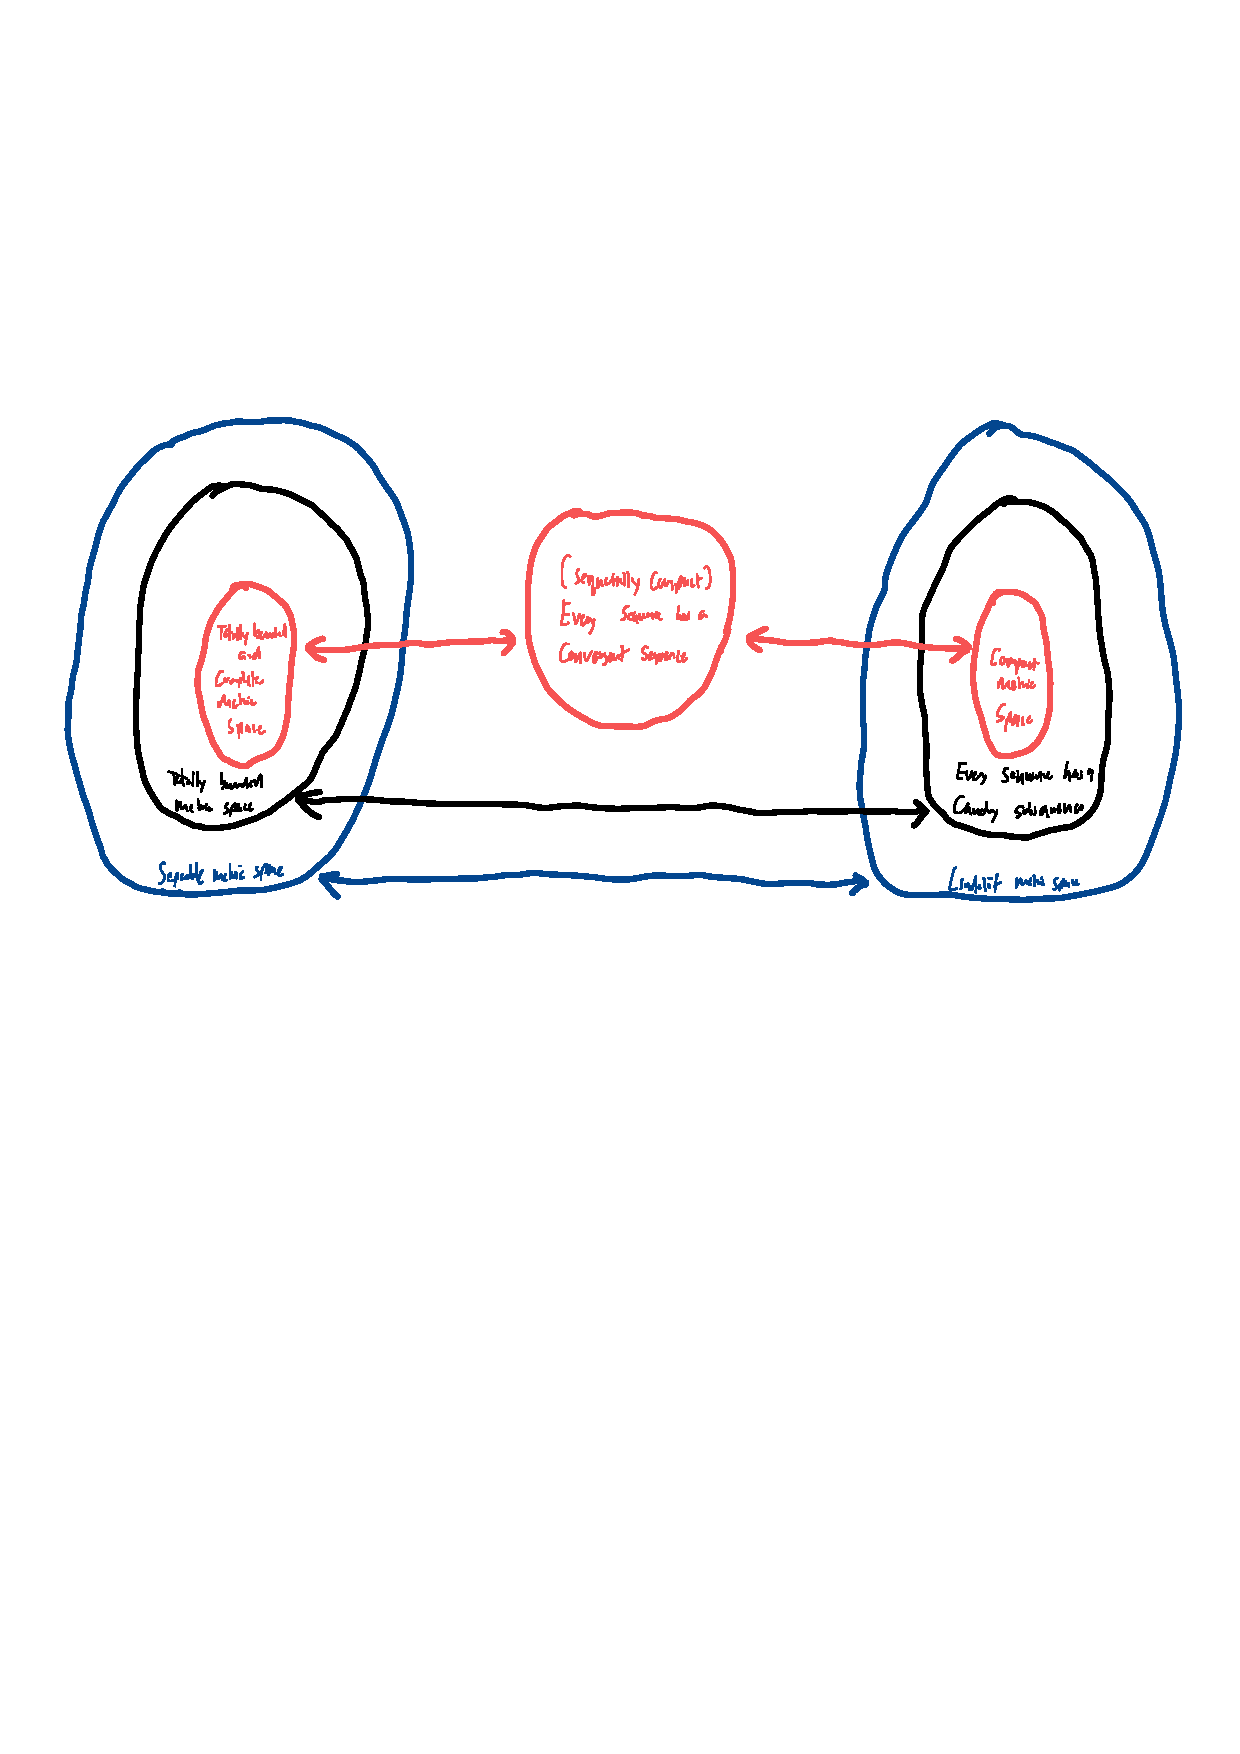
\includegraphics[height=10cm, width=15cm]{Compactness-Characterisation}
\caption{Relationships for compact metric spaces.}
\end{figure}
\end{center}


\lecture{23}{Compactness in Topological Spaces}
\section{Compactness}
\subsection{Compactness in Topological Spaces}
\begin{lemma}Every compact metric space is totally bounded and complete.
\end{lemma}

\begin{theorem}Let X be a compact topological space and let $A \subseteq X$. If A is closed in X, then A is compact in X.
\end{theorem}

\begin{remark}The intuition that we need $A \subseteq X$ to be closed is that $A^c$ will be open and hence for an open covering of A denoted by $\{U_i\}_{i \in I}$, we have that $\{U_i\}_{i \in I} \cup A^c$ is an open cover of X. Since X is compact, we can find a finite subcover for X and as a result, a finite subcover for A too.
\end{remark}

\begin{lemma}Let S be a compact subset of a Hausdorff topological space X. Then, for every $x \in $ X \textbackslash S, there exists disjoint open neighbourhoods U of x and V of S.
\end{lemma}


\begin{theorem}Let X be a Hausdorff topological space and let $A \subseteq X$. If A is compact in X, then A is closed in X.
\end{theorem}

\begin{remark}The intuition is that since X is Hausdorff, we can construct a collection of neighbourhoods to cover points in A and another collection to cover points not in A that do not intersect. Then since A is compact, we can find a finite subcover of A and we can find a finite set for the points not in A. The intersection of these sets not covering A will be open and hence the complement of A is open, meaning that A is closed.
\end{remark}

\begin{theorem}(Characterisation of compact topological spaces). Let $(X, \tau)$ be a topological space. The space X is compact if and only if for a family of closed sets of X $\{F_j\}_{j \in J}$, we have that 
$$
\bigcap_{j \in J}F_j \neq \emptyset.
$$
\end{theorem}


\begin{definition}(Regular Space). A topological space is called regular if every closed subset $A \subset X$ and a point $x \not \in A$ admits disjoint open neighbourhoods.
\end{definition}

\begin{definition}(Normal Space). A topological space is called normal if every disjoint nonempty closed subsets of X admits disjoint open neighbourhoods.
\end{definition}

\begin{theorem}Every compact Hausdorff space is normal.
\end{theorem}

\begin{remark}Compact subsets of a non-Hausdorff topological space need not be closed.
\end{remark}

\begin{proposition}Any finite union of compact subsets of a topological space is compact.
\end{proposition}

\begin{proof}Use induction. For n=2, let $U_1, U_2 \subseteq X$ be compact subsets. Let C be an open cover of $U_1 \cup U_2$. Then C is an open cover of $U_1$ and $U_2$. Since they are compact, there exists a countable subcovers $U_1 \subseteq C_1$ and $U_2 \subseteq C_2$. We have that $U_1 \cup U_2 \subseteq C_1 \cup C_2$ is a countable subcover. 
\end{proof}

\begin{proposition}Every intersection of compact subsets of a Hausdorff space is compact.
\end{proposition}

\begin{proof}Use induction. For n=2, let A and B be compact subsets of the Hausdorff space X. Then A and B must be closed sets. Their intersection is closed. $A \cap B$ is a closed subset of the compact sets A and B, hence it is compact as closed subsets of a compact set is compact.
\end{proof}


\begin{proposition}A discrete topological space is compact if and only if it is finite.
\end{proposition}

\begin{proposition}Any non-empty subset with the cofinite topology is compact.
\end{proposition}

\begin{theorem}(Extreme value theorem). Let $f:X \rightarrow \mathbb{R}$ be a continuous function where X is a compact topological space. Then f is bounded and, moreover, f attains its maximum value and minimum value.
\end{theorem}

\begin{proof}X is compact so $f(X) \subseteq \mathbb{R}$ is compact. Recall that a set in $\mathbb{R}^N$ is compact if and only if it is closed and bounded. Hence $f$ is closed and bounded in $\mathbb{R}$. Hence f is bounded.
\newline
Now recall 2 things
\begin{enumerate}
\item Every bounded set admits a supremum/infimum.
\item Every closed set contains its supremum/infimum.
\end{enumerate}
Hence f(X) admits a supremum and infimum in $\mathbb{R}$ contained in itself. Hence f attains its maximum and minimum value.
\end{proof}

\begin{theorem}Let $f:X \rightarrow Y$ where X is a compact metric space. Then any continuous function f is uniformly continuous.
\end{theorem}

\begin{definition}($T_3$-Space). A topological space is a $T_3$ space if it is a $T_1$ space and regular.
\end{definition}

\begin{definition}($T_4$-Space). A topological space is a $T_4$ space if it is a $T_1$ space and normal.
\end{definition}

\begin{lemma}Every $T_4$ space is a $T_3$ space.
\end{lemma}

\subsection{Separation Axioms}



\begin{figure}
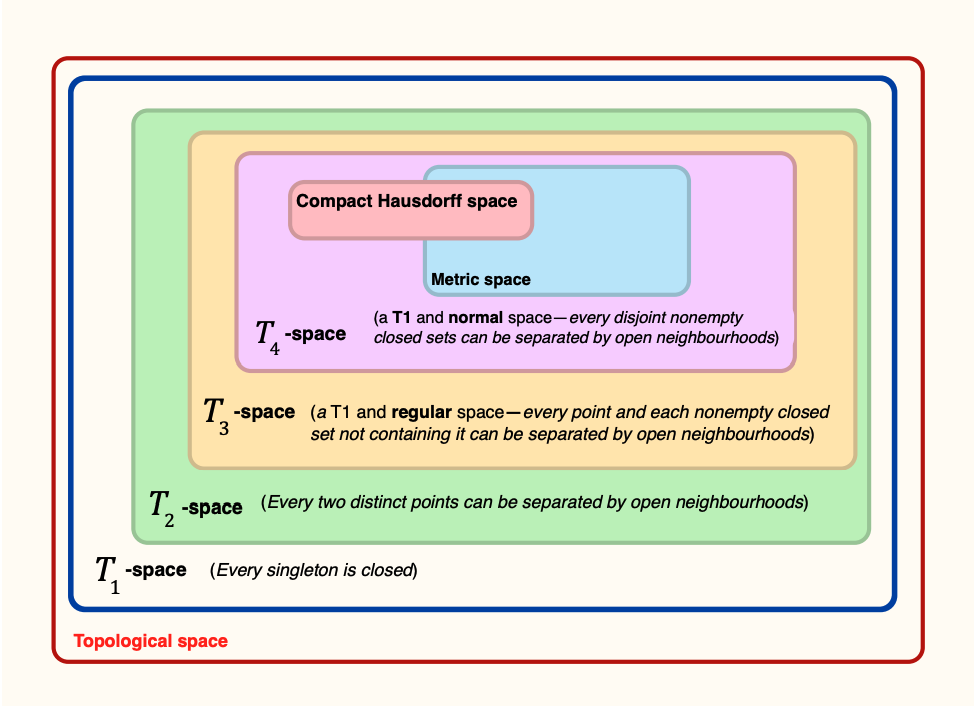
\includegraphics[height=14cm, width=17cm]{Separation-Axioms}
\caption{Separation Axioms.}
\end{figure}

\subsection{Characterisation of regular/normal spaces}
\begin{proposition}(Characterisation of a normal space). A topological space X is normal if and only if each open neighbourhood of any nonempty closed subset A of X contains the closure of an open neighbourhood of A.
\end{proposition}

\begin{proposition}(Characterisation of a regular space). A topological space X is regular if and only if each open neighbourhood of any $x \in X$ contains the closure of an open neighbourhood of x. 
\end{proposition}


\subsection{Important examples of $T_4$ spaces}
\begin{theorem}Every metric space is a $T_4$ space.
\end{theorem}

\begin{proposition}Let X be a Hausdorff space and let S be any compact subset of X.
\begin{enumerate}
\item For every $x \in X$ \textbackslash S, there exist disjoint open neighbourhoods U of x and V of S.
\item The compact subset S is closed.
\end{enumerate}
\end{proposition}

\begin{remark}Compact subsets of a non-Hausdorff space need not be closed.
\end{remark}

\begin{theorem}Every compact Hausdorff space is a $T_4$ space.
\end{theorem}

\begin{corollary}A compact space is a $T_2$-space if and only if it is a $T_3$-space if and only if it is a $T_4$ space.
\end{corollary}

\subsection{Baire Category Theorem Revisited}
\begin{theorem}Every compact Hausdorff space is a Baire space.
\end{theorem}


\lecture{24}{Urysohn's Lemma}
\section{Compactness}
\subsection{Urysohn's Lemma}

Urysohn's lemma is useful for us to establish whether is a topological space is normal. 
\begin{theorem}(Urysohn's Lemma). Let X be a topological space. X is a normal space if and only if for every non-empty closed set A and B that are disjoint, there exists a continuous function $f: X \rightarrow [0, 1]$ such that 
$$
\begin{cases}
f = 0 & \text{on A} \\
f = 1 & \text{on B}
\end{cases}
$$
\end{theorem}

\begin{lemma}A topological space is normal if and only if any two disjoint closed subsets can be separated by a continuous function.
\end{lemma}

\begin{remark}Separated here refers to the fact that the closure of two sets are disjoint.
\end{remark}

Uryson's lemma is useful for formulating conditions for a topological space to be metrizable. Furthermore, Urysohn's lemma is useful as all metric spaces and all compact Hausdorff spaces are normal.

\begin{remark}We can extend from having an interval of [0, 1] to an interval of [a, b] where $a < b$. We have that $\tilde{f}:X \rightarrow [a,b]$ such that $\tilde{f} = a$ on A and $\tilde{f} = b$ on B.
\end{remark}

\lecture{25}{Tietze-Urysohn Extension Theorem}
\section{Compactness}
\subsection{Revision from analysis on sequences of functions}
We look at sequences of functions
$
f_n: D \rightarrow \mathbb{K}^N
$
with domain $D \subseteq \mathbb{K}^d$ and $n \in \mathbb{N}$. If we fix $x \in D$, we then have that $f_n(x)$ is a sequence in $\mathbb{K}^N$.

\begin{definition}(Pointwise Convergence). We say that the sequence of functions $f_n$ converges pointwise to f on D if for all $x \in D$, the sequence $\{f_n(x)\}$ converges to f(x) as $n \rightarrow \infty$. That is, for all $x \in D$ and for all $\epsilon > 0$, there exists $n_{\epsilon,x} \geq 1$ such that
$$
||f_n(x) - f(x)|| < \epsilon
$$
for all $n \geq n_{\epsilon,x}$.

In other words, we have that
$$
f(x) = \Lim{n \rightarrow \infty}f_n(x)
$$
for all $x \in D$. We write $f_n \rightarrow f$ pointwise.
\end{definition}

\begin{definition}(Uniform Convergence). We say $f_n \rightarrow f$ uniformly on D if for every $\epsilon > 0$, there exists $n_{\epsilon} \in \mathbb{N}$ such that
$$
||f_n(x) - f(x)|| < \epsilon
$$
for all $n > n_{\epsilon}$ and all $x \in D$. We say that $f_n(x) \rightarrow f(x)$ uniformly with respect to $x \in D$.
\end{definition}


\begin{definition}(Supremum Norm). Let $f: D \rightarrow \mathbb{K}^N$ be a function. We define its $\textbf{supremum norm}$ by
$$
||f||_{\infty, D} = \sup_{x \in D}||f(x)||.
$$
\end{definition}

\begin{lemma}The supremum norm of a function is finite if and only if f is a bounded function.
\end{lemma}

\begin{proposition}(Characterisation of uniform convergence). Let $f_n: D \rightarrow \mathbb{K}^N$ be functions. Then $f_n \rightarrow f$ uniformly on D if and only if $||f_n - f||_{\infty, D} \rightarrow 0$ as $n \rightarrow \infty$.
\end{proposition}

\begin{definition}(Absolute Convergence for series of functions). Let $g_k: D \rightarrow \mathbb{K}^N$ be a $\textbf{sequence}$ of functions, where $D \subseteq \mathbb{K}^d$. The series $\sum_{k=0}^{\infty}g_k$ is called absolutely convergent on D if for every $x \in D$, the series $\sum_{k=0}^{\infty}g_k(x)$ converges absolutely. In other words,
$$
\sum_{k=0}^{\infty}||g_k(x)||_{\infty, D}
$$
converges in $\mathbb{R}$ for all $x \in D$.
\end{definition}

\begin{remark} So what this means is that we fix $x \in D$ and then we get a series of vectors by evaluating each function at x. Recall that to check for convergence of a series of vectors, you look at the series of norms and see does that converge in $\mathbb{R}$. Then see does the series of norms converge in $\mathbb{R}$ for every $x \in D$. If it does, then it is absolutely convergent.
\end{remark}

\begin{definition}(Uniform Convergence for series of functions). Let $g_k: D \rightarrow \mathbb{K}^N$ be a $\textbf{sequence}$ of functions, where $D \subseteq \mathbb{K}^d$. If the sequence of $\{f_n\}$ of partial sums converges uniformly on D, where $f_n(x) = \sum_{k=0}^{n}g_k(x)$ for all $x \in D$, the series $\sum_{k=0}^{\infty}g_k$ converges uniformly.
\end{definition}

\begin{remark} A series converges if the series of partial sums converges. However, we want uniform convergence, so we need to have that the series of partial sums to converge uniformly on D. So the sequence of partial sums is a sequence of functions $\{f_n\}$. Recall that the uniform convergence of a sequence of functions is when the supremum norm $||f_n - f||_{\infty,D} \rightarrow 0$ as $n \rightarrow \infty$.
\end{remark}


We can now introduce a criterion to check for uniform convergence of a series.

\begin{theorem}(Weierstrass M-Test). Let $g_n: D \rightarrow \mathbb{K}^N$ be a sequence of functions. If
$$
\sum_{k=0}^{\infty}||g_k||_{\infty, D}
$$
converges, then the original series
$$
\sum_{k=0}^{\infty}g_k
$$
converges absolutely and therefore uniformly on D.
\end{theorem}

\begin{remark} Here, we look at the series of supremum norms of each function $g_k$, which is finding the largest value of $g_k(x)$ for all $x \in D$. We get a series of non-negative numbers when we take the supremum norms and if this series of non-negative numbers converges (where we can use many of the tests for non-negative series), then the series converges absolutely and uniformly on the domain D. 
\end{remark}

\subsection{Tietze-Urysohn Extension Theorem}

The Tietze-Urysohn extension theorem is useful to help us in determining whether is a space a normal space.

\begin{theorem}(Tietze-Urysohn Extension Theorem). Let X be a normal topological space and let Y be a closed subspace of X. Let $f:Y \rightarrow \mathbb{R}$ be a bounded and continuous function on Y. Then there exists a function $h:X \rightarrow \mathbb{R}$ that is bounded and continuous on X such that $h|_Y = f$.
\end{theorem}

\begin{proof}(Sketch). We denote $f: Y \rightarrow \mathbb{R}$ to be a bounded and continuous function on Y where $C_0 \coloneqq ||f||_{\infty,Y} = \sup_{y \in Y}|f(y)|$. We will construct a bounded and continuous function $h: X \rightarrow \mathbb{R}$ such that $h|Y = f$.
\newline
To construct h, we define 
$$
h = \sum_{n=0}^{\infty}g_n
$$
where $g_n:X \rightarrow \mathbb{R}$ are bounded and continuous functions. We then construct the sequence 
$$
h_n = \sum_{k=0}^{\infty}g_k
$$
for all $n \in \mathbb{N}$. We require $g_n$ to satisfy 2 properties 
\begin{enumerate}
\item $||g_n||_{\infty,X} \leq C_0\frac{2^n}{3^n+1}$ for all $n \geq 0$,
\item $||f - \sum_{k=0}^{\infty}g_k||_{\infty, Y} \leq C_0\frac{2^{n+1}}{3^{n+1}}$ for all $n \geq 0$.
\end{enumerate}

Property 1 ensures that our function h is the sum of a uniformly convergent sequence $\{h_n\}_{n \geq 1}$ and hence h will be continuous by invoking the Weierstrass M-test.
\newline
Property 2 ensures the uniform limit of h coincides with f so that h=f on Y by letting $n \rightarrow \infty$.
\newline
We construct the sequence $\{g_n\}_{n \geq 1}$ by constructing the closed sets where $f(y) \leq |\frac{C_0}{3}$ which will be closed in Y and also be closed in X due to Y being closed. We can then apply Urysohn's lemma to construct $g_0$. We repeat the step inductively to construct our sequence $\{g_n\}_{n \geq 1}$.
\end{proof}

\lecture{26}{Connected Spaces}
\section{Connected Spaces}
\section{Connected Spaces}
\subsection{Connected Spaces}

\begin{definition}(Separation). A separation of a topological space X is a pair $U, V$ of disjoint non-empty open subsets of X such that
\begin{enumerate}
\item $U \cup V = X$
\item $U \cap V = \emptyset$
\item $U \neq \emptyset$ and $V \neq \emptyset$ 
\item $U, V \in \tau$
\end{enumerate}
\end{definition}
\begin{definition}(Disconnected). Let X be a topological space. We say that X is separated/disconnected if it can be broken up into 2 disjoint non-empty open subsets of X.
\end{definition}

\begin{definition}(Connected). A topological space X is connected if there is no separation of X.
\end{definition}

\begin{theorem}(Clopen set criterion for Connectdness). X is connected if and only if the only clopen subsets of X is the empty set and X.
\end{theorem}

\begin{remark}To show a topological space is not connected, find a clopen set that is not $\emptyset$ or X.
\end{remark}

\begin{definition}(Connected subspace). Let X be a topological space. A subset $E \subseteq X$ is called a connected subspace if E is connected in the relative topology $\tau_E$; i.e. there is no separation with open sets from $\tau_E$
\end{definition}

\begin{remark}Connectdness is a topological property which is preserved by homeomorphisms. This is because it is formulated entirely by open space.
\end{remark}

\begin{remark}To show that 2 spaces are $\textbf{not}$ homeomorphic, we need to show that one space is not connected/compact.
\end{remark}

\begin{theorem}Let X and Y be topological spaces. Let f be a continuous function. If X is connected, then $f(X)$ is a connected subset of Y.
\end{theorem}

\begin{remark}This relaxes the condition for f to be a homeomorphism as f does not need to be a bijection.
\end{remark}

\begin{corollary}If X and Y are topoloigcal spaces and $f:X \rightarrow Y$ is a homeomorphism between X and Y, then if X is connected, then Y is connected.
\end{corollary}

\begin{theorem}Let X be a topological space and let $A \subseteq X$. If the subspace A is connected, then the closure $\overline{A}$ is also connected.
\end{theorem}

\begin{definition}(Totally disconnected). A topological space in which singletons are the only connected subsets is called totally disconnected.
\end{definition}

\begin{remark}A totally disconnected space does not imply a discrete space.
\end{remark}

\begin{theorem}Let X and Y be topological spaces. If for every $x \in X$, we have that X \textbackslash $\{x\}$ is connected with regards to the subspace topology, and if there exists a $y \in Y$ such that $Y$ \textbackslash $\{y\}$ is disconnected with respect to the subspace topology, then X is not homeomorphic to Y.
\end{theorem}

\lecture{27}{Applications of Connected Spaces}
\section{Connected Spaces}
\subsection{Applications of Connected Spaces}

\begin{theorem}(Intermediate Value Theorem). Let $f:X \rightarrow \mathbb{R}$ be a continuous function where X is a connected topological space. If $a,b \in X$, then for all M between $f(a)$ and $f(b)$, there exists a $c \in X$ such that $f(c) = M$.
\end{theorem}

\begin{theorem}All intervals of $\mathbb{R}$ with the usual topology on $\mathbb{R}$ are connected and these are the only connected subsets of $\mathbb{R}$.
\end{theorem}

The arbitrary union of connected topological spaces need not be connected. However, if we have a point common to all the connected spaces, then the union is indeed connected. We introduce a sufficient condition for the union of connected spaces to be connected.
\begin{theorem}(Common point criterion for connected unions). Let X be a topological space and let $\{A_i\}_{i \in I}$ be an arbitrary collection of connected topological spaces. If 
$\bigcap_{i \in I}A_i \neq \emptyset$ then $\bigcup_{i \in I}A_i$ is connected.
\end{theorem}

We can develop a similar result to the theorem above.

\begin{theorem}Let $\{E_j\}_{j \in J}$ be a family of connected subsets of a topological space X such that $E_j \cap E_k \neq \emptyset$ for all $j, k \in J$. Then $$\bigcup_{j \in J}E_j$$ is also connected.
\end{theorem}

\lecture{28}{Path Connectdness}
\section{Connected Spaces}
\subsection{Path Connectdness}
\begin{definition}(Connected Component). Let X be a topological space and pick a point $x \in X$. The connected component of $x \in X$, denoted by C(x), is the union of all connected subsets of X that contains x.
\end{definition}

\begin{remark}We have that 
\begin{enumerate}
\item C(x) is connected.
\item C(x) is the largest connected subset of X that contains x.
\end{enumerate}
\end{remark}

\begin{theorem}Any 2 connected components of a topological space X either coincides or are disjoint.
\end{theorem}

\begin{theorem}The connected component of X forms a partition of X into maximal connected subsets, that is, 
$$
X = \bigcup_{x \in X}C(x)
$$
where for any $x, y \in X$, we have either that
\begin{enumerate}
\item $C(x) = C(y)$ or
\item $C(x) \cap C(y) = \emptyset$.
\end{enumerate}
\end{theorem}

\begin{definition}(Totally disconnected). A topological space is totally disconnected if the singletons are the only connected subsets.
\end{definition}

\begin{lemma}Every discrete/countable metric space is totally disconnected.
\end{lemma}

\begin{lemma}If E is a connected subset of a topological space, then $\bar{E}$ is also connected.
\end{lemma}

\begin{theorem}Every connected component of a topological space is closed.
\end{theorem}

\begin{definition}(Path). Let $x_0, x_1 \in A$. A path in X from $x_0$ to $x_1$ is a continuous function $\gamma$ such that 
$$
\gamma:[0, 1] \rightarrow X
$$
such that $\gamma(0) = x_0$ and $\gamma(1) = x_1$.
\end{definition}

\begin{definition}(Path-Connected). The space X is called path-connected if for every $x_0, x_1 \in X$, there exists a path from $x_0$ to $x_1$.
\end{definition}

\begin{lemma}The relation "there is a path from x to y" is an equivalence relation which satisfies the properties of
\begin{enumerate}
\item Reflexive,
\item Symmetric,
\item Transitive.
\end{enumerate}
\end{lemma}

\begin{definition}(Path Components). The equivalent classes corresponding to the above relation are called the path components of X.
\end{definition}

\begin{definition}(Path-Connected Space). A topological space is called path-connected if there is one path component, that is, any 2 points of X can be joined by a path in X.
\end{definition}

\begin{remark}Path components of X are the maximal path-connected subsets of the space X.
\end{remark}

\begin{remark}The path components of a space need not be open. Path components need not coincide with the connected components.
\end{remark}

\begin{lemma}A fixed path component always lies within a necessarily unique connected component.
\end{lemma}

\begin{theorem}A path connected space X is connected.
\end{theorem}

\begin{lemma}An open ball in $\mathbb{R}^d$ for $d \geq 2$ is path connected and therefore connected.
\end{lemma}

\begin{remark}A connected space does NOT imply a path-connected space.
\end{remark}

\begin{lemma}Only 1 connected component contains the path component A.
\end{lemma}

\begin{corollary}Let X be a topological space. Then each connected component of X is an union of path components of X.
\end{corollary}
\begin{remark}Path components of a topological space need not coincide with the connected components if X is locally path-connected.
\end{remark}

\begin{definition}(Cut point). A point p of a topological space is called a cut point if $X - \{p\}$ is not connected.
\end{definition}

\begin{remark}To see whether 2 spaces are homeomorphic, you can count to see if there number of non-cut points are the same in both spaces. Homeomorphism preserves the connected structure of the space and hence the number of cut points.
\end{remark}


\lecture{29}{Contraction Mapping Theorem}
\section{Contraction Mapping Theorem}
\section{Contraction Mapping Theorem}
\subsection{Contraction Mapping Theorem}
The purpose of the contraction mapping theorem is to determine what are the sufficient conditions for the existence of fixed points for mappings.

\begin{definition}(Fixed point). Let (X, d) be a metric space and $\phi:X \rightarrow X$  be a function. Then $x \in X$ is a fixed point of $\phi$ if $\phi(x) = x$.
\end{definition}

\begin{definition}(Contraction). A map $\phi:X \rightarrow X$ is called a contraction if there exists $c \in (0,1)$ such that 
$$
d(\phi(x), \phi(y)) \leq cd(x,y)
$$
for all $x, y \in X$.
\end{definition}

\begin{lemma}If $\phi:X \rightarrow X$ is a contraction, then there is at most one fixed point for $\phi$.
\end{lemma}

\begin{theorem}(Contraction Mapping Theorem). Every contraction $\phi$ on a complete metric space (X, d) admits a unique fixed point $x_*$. Moreover, this fixed point can be constructed as follows, pick an arbitrary $x \in X$ and define $x_n = \phi(x_{n-1})$. Then, $\lim_{n \rightarrow \infty}x_n = x_*$.
\end{theorem}
\begin{proof}(Sketch). We only need to show existence of a fixed point as from the previous lemma, we are guaranteed the uniqueness of a fixed point.
\newline
1) Construct a sequence $x_{n+1} = \phi^n(x_0)$ and show that $\{x_n\}_{n \geq 1}$ is a Cauchy sequence. By the completion of X, $\{x_n\}_{n \geq 1}$ converges to a point $x_*$ in X.

2) Show that $x_*$ is the fixed point by using triangle inequality, definition of contraction, and taking limits.
\end{proof}

\subsection{Applications of the Contraction Mapping Theorem}

\begin{definition}(Lipschitz continuous). We assume that F is Lipschitz continuous in the first variable, there exists a constant $L > 0$ such that
$$
|F(x,t) - F(y,t)| \leq L|x-y|
$$
for $x, y \in \overline{B}(\psi,r)$ and every $t \in [0,T]$.
\end{definition}

\begin{theorem}(Cauchy-Picard Theorem). Let $U$ be an open subset of $\mathbb{R}^n$. Fix $\psi \in U$. For $T > 0$, let $F: U \times [0,T] \rightarrow \mathbb{R}^n$ be a continuous functions. Choose $r > 0$ small enough such that the closed ball $\overline{B}(\psi, r) \subseteq U \subseteq \mathbb{R}^n$. By continuity of F and compactness of $\overline{B}(\psi, r) \times [0,T]$, we have 
$$
M \coloneqq \sup\{|F(x,t)|: (x,t) \in \overline{B}(\psi;r) \times [0,T]\} < \infty.
$$
We assume that F is Lipschitz continuous.
\newline
Suppose the above condition hold. Then, there exists $\beta \in [0,T]$ such that the following initial value problem has a unique solution u on $[0, \beta]$:

$\frac{du}{dt} = F(u(t), t)$ for $0 \leq t \leq \beta$, \\ 
$u(0) = \psi.$


Furthermore, $\beta$ depends only on r, M and the Lipschitz constant L.
\end{theorem}


\lecture{30}{Normed Vector Space}
\section{Hilbert Spaces}
\section{Hilbert Spaces}
\subsection{Normed Vector Space}
\begin{proposition}(Continuity of the norm). Let $(E, ||.||)$ be a normed vector space. Then the norm $||.||: E \rightarrow \mathbb{R}$ is a continuous function.
\end{proposition}
\begin{proof} Since E is a normed vector space, then it is also a metric space. Recall that to show a function is continuous, we can show it is sequentially continuous for a metric space.
\end{proof}

\begin{proposition}(Continuity of inner product). Let E be an inner product space. Then the inner product $\langle .,. \rangle: E \times E \rightarrow \mathbb{K}$ is continuous with respect to the induced norm.
\end{proposition}

\begin{proposition}(Paralellogram identity). Let $(E, \langle .,. \rangle)$ be an inner product space and let $||.||_{\infty}$ be the induced norm. Then
$$
||u+v||^2 + ||u-v||^2 = 2(||u||^2 + ||v||^2)
$$
for all $u, v \in E$.
\end{proposition}

\begin{lemma}Let $||.||$ be a norm on a vector space E satisfying the parallelogram identity. Then there exists an inner product on E inducing the norm $||.||$ where $\langle .,. \rangle = \sqrt{||.||}$.
\end{lemma}

\begin{theorem}(Cauchy-Schwarz Inequality). Let E be an inner product space with an inner product $\langle .,. \rangle)$. Then 
$$
| \langle u, v \rangle | \leq ||u||.||v||
$$
for all $u,v \in E$ with equality if and only if u and v are linearly dependent.
\end{theorem}

\lecture{31}{Projections}
\section{Hilbert Spaces}
\subsection{Projections}
\begin{definition}(Distance of a set). Let $S \subset X$ where X is a $\textbf{normed space}$. For every $x \in X$, we define the distance of the point x to the set S itself as 
$$
d(x,S) = \inf_{s \in S}||x - s||.
$$
\end{definition}

\begin{lemma}Let $S \subset X$ where X is a $\textbf{normed space}$. Then for every $x \in X$, $d(x,S) = 0$ if and only if $x \in \overline{S}$.
\end{lemma}

\begin{definition}(Projection). Let E be a normed vector space and M be a $\textbf{non-empty closed}$ subset of E. We define the set of projections for a point $x \in E$ onto M by
$$
P_M(x) = \{m \in M: ||x-m|| = dist(x,M) = inf\{||x-y||: y \in M\}\}.
$$
\end{definition}

\begin{remark}If the non-empty closed subset $M \subset E$ is not a convex subset of the plane, then $P_M(x)$ may contain more than one point.
\end{remark}

\begin{definition}(Proximal). The set M is called proximal if the set $P_M(x)$ is non-empty for each $x \in X$.
\end{definition}

\begin{definition}(Chebychev set). A subset S of X is called a Chebychev set if for every $x \in X$, the set $P_M(x)$ contains a unique point.
\end{definition}

\begin{lemma}Let X admit a Chebychev subset S, then we can define a function $\phi:X \rightarrow S$ from $x \rightarrow P_S(x)$.
\end{lemma}

\begin{proposition}Every Chebychev set in a normed space is proximal.
\end{proposition}

\begin{proposition}A necessary condition for a subset S to be proximal is for S to be closed.
\end{proposition}

\begin{proposition}Every nonempty closed subset of a finite-dimensional normed vector space is proximal.
\end{proposition}

\begin{remark}Being closed is also a sufficient condition for a set to be proximal in $\textbf{finite-dimensional}$ normed spaces. This does not hold for an infinite-dimensional normed space.
\end{remark}

\begin{proposition}Let X be a normed space. Every compact subset of X is proximal but not necessarily Chebychev.
\end{proposition}

\begin{proposition}Every nonempty closed subset $M \subset \mathbb{R}^n$ with the Euclidean norm $||.||$ is proximal.
\end{proposition}

\begin{definition}(Convex set). A set M is convex if for all $\lambda \in [0,1]$, we have that 
$$
\lambda x + (1-\lambda)y \in M
$$
for all $x,y \in M$.
\end{definition}

\begin{theorem}(Existence and uniqueness of projection onto a convex set). Let H be a finite-dimensional Hilbert space and $M \subset H$. Then, M is a Chebychev set if and only if M is closed and convex. That is, for all $x \in X, P_M(x)$ contains a unique point. 
\end{theorem}

\begin{theorem}(Characterisation of projection). Let H be a Hilbert space and M be a nonempty, closed, and convex subset of H. Then for a point $m_x \in M$, the following assertions are equivalent:
\begin{enumerate}
\item A point $m_x \in M$ coincides with the projection $P_M(x)$ of x onto M i.e. $m_x = P_M(x)$;
\item $Re\langle x - m_x, m - m_x \rangle \leq 0$ for all $m \in M$.
\end{enumerate}
\end{theorem}

\begin{remark}By convexity of M, we expect the angle between x and a projection point $m_x$ compared to all other points to be larger or equal to $\pi/2$.
\end{remark}

\begin{definition}(Vector subspace). Let V be the vector space over the field $\mathbb{K}$ and let W be a subset of V. Then W is a vector subspace if for all $x, y \in W$ and for all $\alpha, \beta \in \mathbb{K}$, we have that $\alpha x + \beta y \in W$.
\end{definition}

\begin{proposition}For a $\textbf{normed vector space}$, we have that \\

Normed Vector Space $\supset$ Proximal Set $\supset$ Chebychev Set $\supset$ Nonempty, closed, and convex subset.
\end{proposition}

\begin{proposition}For an $\textbf{inner product space}$, we have that \\

Inner Product Space $\supset$ Closed Vector Space $\supset$ Proximal Subspace $\leftrightarrow$  Chebychev Subspace $\supset$ Complete Subspace
\end{proposition}

\begin{proposition}For an $\textbf{Hilbert space}$, we have that \\

Hilbert Space $\supset$ Proximal Subspace $\leftrightarrow$  Chebychev Subspace $\leftrightarrow$ Complete Subspace $\leftrightarrow$ Closed Vector Subspace

\end{proposition}

\lecture{32}{Orthogonal Complements}
\section{Hilbert Spaces}
\subsection{Orthogonal Complements}

Let M be a nonempty subset of an inner product space $(X, \langle .,. \rangle)$. Recall that the definition of a projection is 
$
P_M(x) = \{m \in M: ||x-m|| = dist(x,M) = inf\{||x-y||: y \in M\}\}.
$

\begin{definition}(Orthogonal complement). The orthogonal complement of M in X, denoted by $M^{\perp}$, is defined by
$$
M^{\perp} \coloneqq \{x \in X: \langle x,m \rangle = 0 \text{ for all m} \in M\}.
$$
\end{definition}

We want to look at properties of orthogonal complements to help us characterise projections in Hilbert spaces.
\begin{lemma}The orthogonal complement $M^{\perp}$ of M in X is a closed vector subspace of X.
\end{lemma}

\begin{lemma}Let $M^{\perp}$ be the orthogonal complement of M in X. We have that
$$
M^{\perp} = \overline{M}^{\perp} = (span M)^{\perp} = (span \overline{M})^{\perp} = \overline{span M}^{\perp}.
$$
\end{lemma}


\begin{lemma}Every vector $\textbf{subspace}$ M of a Hilbert space is convex.
\end{lemma}

\begin{lemma}Let H be a Hilbert space and let $M \subset H$. For any $x \in H$, we can express as the sum of an element in its projection and orthogonal complement
$$
x = P_M(x) + (x - P_M(x))
$$
where $P_M(x) \in M$ and $(x - P_M(x)) \in M^{\perp}$.
\end{lemma}

\begin{theorem}Let M be a closed subspace of a finite dimensional Hilbert space H. Then M is a Chebychev subspace. Moreover, for every $x \in H$, we have $m_x \in M$ coincides with $P_M(x)$ if and only if $x - m_x \in M^{\perp}$. 
\end{theorem}


\begin{theorem}(Orthogonal complements). Let M be a closed vector subspace of the Hilbert space H. The orthogonal projector $P_M: H \rightarrow M$ satisfies the properties 
\begin{enumerate}
\item $H = M \bigoplus M^{\perp}$ and $M^{\perp \perp} = M$.
\item $P_M:H \rightarrow M$ is a bounded linear operator with $||P_M|| \leq 1$. Moreoever, if M is at least one-dimensional, then $||P_M|| = 1$.
\item $P_M(M^{\perp}) = \{0\}$.
\end{enumerate}
\end{theorem}

\begin{remark}We explain the implications of this theorem.
\begin{enumerate}
\item We can decompose the Hilbert space H into a direct sum of a closed subspace M and its orthogonal subspace $M^{\perp}$. Resultantly, $M \cap M^{\perp} = \{0\}$. Furthermore, any element $x \in H$ can be expressed as the sum of an element in M and an element in $M^{\perp}$. In particular, $x = P_M(x) + (x - P_M(x))$ where $P_M(x) \in M$ is the projection and $(x - P_M(x)) \in M^{\perp}$. Finally, we generally have the case that $M \subset M^{\perp \perp}$ but for closed sets in Hilbert spaces, we have equality.
\item The projection operator $P_M$ has a norm of 1 for any non-trivial closed subspaces M. For $||P_M|| \leq 1 \leftrightarrow ||P_Mx|| \leq ||x||$ for all $x \in H$, so the norm of the projection is less than the norm of the vector.
\item The projection of any element in $M^{\perp}$ onto M is the zero vector.
\end{enumerate}
\end{remark}

\begin{lemma}Let $S \subset H$ where H is a Hilbert space and S is a closed subspace. Then, $S^{\perp}$ is a complete subspace.
\end{lemma}

We now change the focus from Hilbert spaces to inner product spaces, whereby a closed vector subspace $\textbf{does not}$ imply a Chebychev subspace.
\begin{theorem}(Pre-projection theorem). Every proximal vector subspace M of an inner product space X is a Chebychev subspace. Moreover, for every $x \in X$, we have $m_x \in M$ coincides with $P_M(x)$ if and only if $x - m_x \in M^{\perp}$. Furthermore, the orthogonal projector $P_M:X \rightarrow M$ satisfies the properties of:
\begin{enumerate}
\item $X = M \bigoplus M^{\perp}$ and $M^{\perp \perp} = M$.
\item $P_M:X \rightarrow M$ is a bounded linear operator with $||P_M|| \leq 1$. Moreoever, if M is at least one-dimensional, then $||P_M|| = 1$.
\item $P_M(M^{\perp}) = \{0\}$.
\end{enumerate}
\end{theorem}

\begin{theorem}Let X be an inner product space over $\mathbb{K}$. Let M be a vector subspace of X. Then M is a closed and convex subset of X. Furthermore, every proximal subspace coinces with a Chebychev subspace.
\end{theorem}

\begin{proposition}(Characterisation for a dense subset in a Hilbert space). A vector subspace M of a Hilbert space H is dense in H if and only if $M^{\perp} = \{0\}$. In particular, $H = \overline{M} \bigoplus M^{\perp}$.
\end{proposition}

\begin{corollary}Suppose that M is a non-empty subset of the Hilbert space H. Then
$$
M^{\perp \perp} \coloneqq (M^{\perp})^{\perp} = \overline{Span(M)}.
$$
\end{corollary}
\lecture{33}{Hilbert Spaces}
\section{Hilbert Spaces}
\subsection{Hilbert Spaces}

\begin{lemma}Any finite-dimensional normed space is complete and separable.
\end{lemma}


\begin{proposition}In a finite-dimensional normed space E, any two norms are equivalent, that is, for every pair of norms $||.||_1$ and $||.||_2$ on E, there exist a positive constant C such that 
$$
C||x||_2 \leq ||x||_1 \leq C||x||_2 
$$
for all $x \in E$.
\end{proposition}

\begin{corollary}(Generalisation of Heine Borel Theorem). In a finite-dimensional normed space, a set is compact if and only if it is closed and bounded.
\end{corollary}

\begin{definition}(Isometric isomorphism). A linear transformation T from a normed space $(X,||.||_X)$ to a normed space $(Y,||.||_Y)$ is called an isometric isomorphism if T is bijective and $||T(x)||_Y = ||x||_X$ for all $x \in X$.
\end{definition}

\begin{theorem}Every finite dimensional inner product spaces is a separable Hilbert space.
\end{theorem}
\begin{proof} Every finite dimensional inner product space has an isometric isomorphism to $\mathbb{K}^N$ with the usual dot product, which itself is a complete inner product space.
\end{proof}

There are 3 types of Hilbert spaces.
\begin{enumerate}
\item Finite dimensional Hilbert spaces.
\item Infinite dimensional separable Hilbert spaces.
\item Infinite dimensional non-separable Hilbert spaces.
\end{enumerate}

\begin{example}The prototype for the separable infinite dimensional Hilbert space is the Hilbert space $\ell_2$ with the inner product $\langle x, y \rangle_{\ell_{2}} = \sum_{j=1}^{\infty}x_j\bar{y}_j$.
\end{example}

\begin{proposition}Every finite-dimensional Hilbert space is separable.
\end{proposition}


\lecture{34}{Orthonormal Sequences}
\section{Hilbert Spaces}
\subsection{Orthonormal Sequences}

\begin{definition}(Orthogonal Vectors). Two vectors $u, v$ of a Hilbert space H are orthogonal if $\langle u, v \rangle = 0.$
\end{definition}


\begin{theorem}(Pythagoras' Theorem). Let $k \geq 2$. If $u_1,...,u_k$ are mutually orthogonal vectors in an inner product space X, then we have 
$$
||\sum_{j=1}^ku_j||^2 = \sum_{j=1}^k||u_j||^2.
$$
\end{theorem}

\begin{definition}(Orthonormal Sequence). A sequence $\{e_j\}_{j \geq 1}$ in a Hilbert space H is called orthonormal if 
$$
\begin{cases}
\langle e_j, e_k \rangle = 0 \quad \text{ if } j \neq k\\
\langle e_j, e_j \rangle = ||e_j||^2 = 1 \quad \text{ for all } j \geq 1. 
\end{cases}
$$
\end{definition}

\begin{definition}(Span). Assume that $\{e_j\}_{j \geq 1}$ is an orthonormal sequence in X. For every $N \geq 1$, let $E_N$ denote the vector space spanned by $e_1,...,e_N$, which we denote by 
$$
E_N = span\{e_1,...,e_N\}.
$$
The finite-dimensional vector space $E_N$ with the induced inner product from X is a Hilbet space.\\
Furthermore, we have that 
$$
span\{e_j\}_{j \geq 1} = \bigcup_{N=1}^{\infty}E_N.
$$

\end{definition}

\begin{lemma}Every complete vector subspace of an inner product space is a Chebychev subspace. Hence, $E_N$ is a Chebychev subspace and any projection onto $E_N$ will be a unique projection.
\end{lemma}

We first look at the representation of a vector in $E_N$. We then look at the representation of a vector in X that is projected onto $E_N$.
\begin{proposition}Let $\{e_j\}_{j \geq 1}$ be an orthonormal sequence in an inner product space $(X, \langle.,.\rangle)$.
\begin{enumerate}
 \item If $v \in E_N = span\{e_1,...,e_N\}$, then $v = \sum_{j=1}^N\langle v, e_j \rangle e_j$ and $||v||^2 = \sum_{j=1}^N|\langle v, e_j \rangle|^2$.

 \item For every $N \geq 1$, the $\textbf{unique}$ projection of $u \in X$ onto $E_N$ is $U_N = \sum_{j=1}^N\langle u, e_j\rangle e_j$ and, moreover, $$||u||^2 = ||u - U_N||^2 + ||U_N||^2.$$
 \end{enumerate}
\end{proposition}

\begin{remark}The first result in the above proposition states that the scalar coefficient $\lambda_j$ of the linear combination of the orthonormal sequence for a given vector v is the inner product of v and corresponding orthonormal vector $e_j$. The second result looks at the unique projection of u onto X and we can decompose u by an element in $E_N$ and its orthogonal complement $E_{N}^{\perp}$ and then apply Pythagoras theorem.
\end{remark}

\begin{lemma}A non-negative series is convergent if and only if the sequence of partial sums is bounded from above.
\end{lemma}
\begin{remark}The sequence of non-negative partial sums is monotonically increasing and hence we only need to show it is bounded in order to show convergence.
\end{remark}

\begin{proposition}(Bessel's Inequality). If $\{e_j\}_{j \geq 1}$ is an orthonormal sequence in an inner product space $(X, \langle .,. \rangle)$, then
$$
\sum_{j=1}^{\infty}|\langle u, e_j \rangle|^2 \leq ||u||^2
$$
for all $u \in X$ where it is a bounded and convergent series.
\end{proposition}

\begin{remark}
Bessel's inequality is a statement of an element u in an inner product space X with respect to an orthonormal sequence.
\end{remark}

We now seek to turn Bessel's inequality to an equality by imposing more assumptions. We will now impose Hilbert spaces rather than inner product spaces.\\

We want to imitate the inner product structure in $\ell_2$ for a Hilbert space.

\begin{proposition}Let $\{e_j\}_{j \geq 1}$ be an orthonormal sequence in a Hilbert space $(H, \langle .,. \rangle)$. If $a = \{a_j\}_{j \geq 1}$ and $b = \{b_j\}_{j \geq 1}$ belong to $\ell_2$, then $u_a = \sum_{j=1}^{\infty}a_je_j$ and $v_b = \sum_{j=1}^{\infty}b_je_j$ are convergent series $\textbf{in H}$ and, moreover, 
$$
\langle u_a, v_b \rangle_H = \langle a,b \rangle_{\ell_{2}} = \sum_{j=1}^{\infty}a_j \overline{b}_j.
$$
\end{proposition}

\begin{proof}(Sketch). We construct the sequence of partial sums and show that it is a Cauchy sequence and by the completeness of H, then it converges where $U_N = \sum_{j=1}^Na_je_j$ for all $N \geq 1$.
\end{proof}

We want to ask the question when does the Fourier Bessel's series $\sum_{j=1}^{\infty}\langle u, e_j \rangle e_j$ converge? This occurs when we upgrade the space from an inner product space to a Hilbert space.

\begin{corollary}Let H be a Hilbert space and let $\{e_j\}_{j \geq 1}$ be an orthonormal sequence in H. Then, for every $u \in H$, the series $\sum_{j=1}^{\infty}\langle u, e_j \rangle e_j$ converges to U in H and $||U|| \leq ||u||.$
\end{corollary}

We now want to ask the question that for a $u \in H$ where H is a Hilbert space, we know from above that the Fourier Bessel series converges to an $U \in H$ which we don't know anything about, when does $U = u$? In order to answer this, we require that the orthonormal sequence $\{e_j\}_{j \geq 1}$ be $\textbf{maximal}$.

\begin{definition}(Maximal/Complete). An orthonormal sequence $\{e_j\}_{j \geq 1}$ in an inner product space X is said to be maximal or complete if whenever u in X satisfies $u \perp e_j$ for each $j \geq 1$, then $u = 0$.
\end{definition}

\begin{theorem}Let $\{e_j\}_{j \geq 1}$ be an orthonormal sequence in a Hilbert space H. The following statements are equivalent.
\begin{enumerate}
\item The vector space span $\{e_j\}_{j \geq 1}$ of finite linear combinations of $e_j$'s is dense in H.
\item The orthonormal sequence $\{e_j\}_{j \geq 1}$ is maximal.
\item For every $u \in H$, the Fourier-Bessel series $\sum_{j=1}^{\infty}\langle u, e_j \rangle e_j$ $\textbf{converges to u in H}$.
\item (Parseval's identity). We have $||u||^2 = \sum_{j=1}^{\infty}|\langle u,e_j \rangle |^2$ for every $u \in H$.
\end{enumerate}
\end{theorem}

\begin{remark}From point 3, we finally managed to get our Fourier-Bessel series to converge to the vector $u \in X$!
\end{remark}

\lecture{35}{Orthonormal Basis}
\section{Hilbert Spaces}
\subsection{Orthonormal Basis}
We have seen that maximal orthonormal sequences are extremely useful to characterise the convergence of the Fourier Bessel series. We now try find the conditions such that we can guarantee the existence of such sequences.
\begin{theorem}Every separable inner product space contains a maximal orthonormal sequence.
\end{theorem}

\begin{remark}We use the Gram-Schmidt procedure on the countable dense subset of the inner product space.
\end{remark}

\begin{lemma}An orthonormal sequence is maximal if and only if it is a countable orthonormal basis.
\end{lemma}

\begin{remark}The term sequence imposes a condition that the cardinality of the set is countable.
\end{remark}

\begin{definition}(Orthogonal/orthonormal). Let H be a Hilbert space. A nonempty subset S of H is called 
\begin{enumerate}
\item $\textbf{Orthogonal set}$ if every distinct vectors x and y in S are orthogonal;
\item $\textbf{Orthonormal set}$ if it is an orthogonal set and $\langle x, x \rangle = ||x||^2 = 1$ for every $x \in S.$
\end{enumerate}
\end{definition}

\begin{definition}(Complete orthonormal basis). A complete orthonormal basis of H is an orthonormal set S such that the span S is dense in H.
\end{definition}

\begin{proposition}An orthonormal set $S \subset H$ is a complete orthonormal basis if and only if for every $u \in H$ that satisfies $u \perp S$, we have that $u = 0$.
\end{proposition}

\begin{corollary}Every separable Hilbert space admits a $\textbf{countable}$ orthonormal basis.
\end{corollary}

\begin{theorem}Let H be a Hilbert space. The following assertions are equivalent:
\begin{enumerate}
\item The Hilbert space H is separable.
\item There exists a countable orthonormal basis for H.
\item Every orthonormal basis of H is countable.
\end{enumerate}
\end{theorem}
\begin{remark}To show that a Hilbert space is not separable, it suffices to find a orthonormal basis that is not countable.
\end{remark}

\begin{theorem}Every separable infinite-dimensional Hilbert space H can be identified with $\ell_2$ via an isometric isomorphism preserving the inner products, meaning that there exists a bijective linear map $T:H \rightarrow \ell_2$ such that $\langle Tu, Tv \rangle_{\ell_{2}} = \langle u, v \rangle$ for every $u, v \in H$. 
\end{theorem}


\lecture{36}{Linear Operators}
\section{Banach Spaces}
\section{Banach Spaces}
\subsection{Linear Operators}
\begin{definition}(Banach space). A normed vector space which is complete with respect to the metric induced by the norm on the space.
\end{definition}

\begin{definition}(Linear Functional). Let X be a vector space. A linear functional T from X to $\mathbb{K}$ is a function $T: X \rightarrow \mathbb{K}$ such that 
\begin{enumerate}
\item $T(x_1, x_2) = T(x_1) + T(x_2)$ for $x_1, x_2 \in X$.
\item $T(\alpha x) = \alpha T(x)$ for all $x \in X$ and $\alpha \in \mathbb{K}$.
\end{enumerate}
\end{definition}
\begin{definition}(Linear Operator). Let X and Y be vector spaces over the $\textbf{same field}$. A linear operator T from X to Y is a function $T: X \rightarrow Y$ such that 
\begin{enumerate}
\item $T(x_1, x_2) = T(x_1) + T(x_2)$ for $x_1, x_2 \in X$.
\item $T(\alpha x) = \alpha T(x)$ for all $x \in X$.
\end{enumerate}
\end{definition}

\begin{definition}(Set of linear operators). We denote the $\textbf{set of all linear operators}$ from X to Y by $\mathcal{L}(X,Y)$.
\end{definition}

\begin{definition}(Bounded Linear Operator). Let T be a linear operator from the normed space $(X, ||.||_X)$ to a normed space $(Y, ||.||_Y)$. T is said to be $\textbf{bounded}$ if there exists an $M > 0$ such that 
$$
||T(x)||_Y \leq M||x||_X
$$
for every $x \in X$. Equivalently, T is bounded if there exists $M > 0$ such that 
$$
||T(x)||_Y \leq M
$$
for all $x \in X$ with $||x|| \leq 1$.
\end{definition}

\begin{lemma}A bounded linear operator maps bounded sets in X to bounded sets in Y.
\end{lemma}

Note that a bounded linear operator is not the same as bounded functions.

\begin{proposition}Let $(X, ||.||_X)$ and $(Y,||.||_Y)$ be normed vector spaces and let T be a linear operator from X to Y. Then the following statements are equivalent:
\begin{enumerate}
\item T is a bounded linear opeartor.
\item T is continuous on X.
\item T is continuous at $0 \in X$.
\end{enumerate}
\end{proposition}

\begin{definition}(Set of bounded linear operators). Let $B(X,Y)$ denote the space of bounded and linear operators from X to Y.
\end{definition}

\begin{remark}The space $B(X,Y)$ is a vector space that is closed under pointwise addition and scalar multiplication.
\end{remark}

\begin{theorem}Let $B(X,Y)$ be the space of bounded and linear operators from X to Y. Then, $B(X,Y)$ is a normed vector space with the norm $||T|| = ||T||_{B(X,Y)} = \sup_{x \in X; ||x|| \leq 1}||T(x)||_Y.$ We call $||T||_{B(X,Y)}||$ the operator norm of T.
\end{theorem}

\begin{remark}Notice that we now have 3 norms involved in the construction of B(X,Y). The norm on X, Y, and the norm on the linear opeator itself. Hence, the norm of a linear operator itself is the smallest value M such that $||T(x)||_Y \leq M$ for all $x \in X$ where $||x|| \leq 1$. Such a supremum exists due to the linear operator T being bounded.
\end{remark}


\begin{lemma}For every $T \in B(X,Y)$, we have that
$$
||T(x)||_Y \leq ||T||||x||_X 
$$
for all $x \in X$.
\end{lemma}

\begin{theorem}If X is a normed vector space and Y is a Banach space, then the space $B(X,Y)$ of bounded linear operators from X to Y is a Banach space where 
$$
||T||_{B(X,Y)} = \sup_{x \in X; ||x|| \leq 1}||T(x)||_Y.
$$
\end{theorem}
\begin{remark}We already knew that B(X,Y) is a normed vector space. By imposing the restriction that Y is now a Banach space, the completeness property allows us to upgrade B(X,Y) to be a Banach space.
\end{remark}


\begin{definition}(Group). A group is a set G, with a binary operation . such that the pair (G,.) satisfies the group axioms of:
\begin{enumerate}
\item Closure.
\item Associativity.
\item Identity element exists.
\item Inverse element exists.
\end{enumerate}
\end{definition}

\begin{definition}(Homomorphism). Let $(G, .)$ and $(H, *)$ be two groups with different group operations. A homomorphism is a function $\phi: G \rightarrow H$ such that
$$
\phi(g . h) = \phi(g) * \phi(h)
$$
for all $g \in G$ and $h \in H$.
\end{definition}

\begin{definition}(Isomorphism). An isomorphism is a homomorphism that is bijective. Two groups are said to be isomorphic if there exists an isomorphism between them.
\end{definition}

\begin{definition}(Topological isomorphism). Let $(X. ||.||_X)$ and $(Y, ||.||_Y)$ be normed linear spaces and let T be a linear operator from X to Y. T is a $\textbf{topological isomorphism}$ if T is an isomorphism and T is continuous with a continuous inverse.
\end{definition}

If the normed linear spaces X and Y are topologically isomorphic, then they are identical for topological purposes (open sets, convergence, continuity etc).

\begin{definition}(Isometric isomorphism). Let $(X. ||.||_X)$ and $(Y, ||.||_Y)$ be normed linear spaces and let T be a linear operator from X to Y. T is a $\textbf{topological isomorphism}$ if T is an isomorphism and T is an isometry, i.e. $||Tx||_Y = ||x||_X$ for all $x \in X$.
\end{definition}

If the normed linear spaces X and Y are isometrically isomorphic, then they are identical for metric purposes (distances, balls etc).


\begin{theorem}Let X be a normed vector space and Y be a Banach space. Let $\{T_n\}_{n \geq 1}$ be a sequence in B(X,Y) that is bounded in B(X,Y)
\end{theorem}

\lecture{36}{Principle of Uniform Boundedness}
\section{Banach Spaces}
\subsection{Principle of Uniform Boundedness}

\begin{theorem}(Principle of uniform boundedness). Let X and Y be Banach spaces. Let $\{T_j\}_{j \in J}$ be a family of bounded linear operators from X to Y, that is,  $T_j \in B(X,Y)$ for each $j \in J$. Assume that $\sup_{j \in J}||T_j(x)|| < \infty$ for every $x \in X$. Then we have that
$$
\sup_{j \in J}||T_j||_{B(X,Y)} < \infty.
$$
\end{theorem}

\begin{proof}(Sketch). As X is a complete metric space, we can express it as a countable union of closed sets. From the Baire Category theorem, that every complete metric space $\textbf{cannot}$ be written as a countable union of nowhere dense sets, then there exists a closed set $E_n$ such that $int(\overline{E}_n) = int(E_n) \neq \emptyset$. We are then able to analyse an open ball in this set and pick a point in the ball that is not the center of the ball. We put a bound on the point by the definition of the set we constructed which the balls sits in. We then use the assumption of pointwise boundedness in addition to the reverse triangle inequality and linearity of the linear operator to derive a constant that bounds the family of linear operators for each point in the open unit ball.
\end{proof}

The principle of uniform boundedness states that if we have a family of pointwise bounded linear operators, i.e. if we fix a point $x \in X$, we can bound the family of linear operators, we can in fact extend this to uniform boundedness. Pointwise boundedness can be expressed as for every $x \in X$, we have that $\sup_{j \in J}||T_j(x)||_Y < \infty$ or equivalently there exists $C_x > 0$ such that 
$$
||T(x)||_Y < C_x
$$
for all $j \in J$.\\ When we refer to uniform boundedness, we refer to the fact that $\sup_{j \in J}||T_j||_{B(X,Y)} < \infty$ which is equivalent to there exists $M > 0$ such that 
$$
||T_j||_{B(X,Y)} \leq M
$$ 
for all $j \in J$, which is equivalent to 
$$
\sup_{x \in X; ||x|| \leq 1}||T_j(x)||_Y.
$$


\lecture{37}{Compactness of sets in separable Hilbert spaces}
\section{Banach Spaces}
\subsection{Compactness of sets in separable Hilbert spaces}
We know that a closed and bounded set is not compact for infinite dimensional metric spaces. An example would be the closed unit ball in a Banach space is not compact. We investigate the characterisation for compact sets in infinite dimensional spaces.
\begin{lemma}(Equi-smallness). Let H be a Hilbert space. If $\{e_k\}_{k \geq 1}$ is an orthonormal sequence in H and $\{u_n\}_{n \geq 1}$ converges to U in H, then for every $\epsilon > 0$, there exists $N \geq 1$ such that
$$
\sum_{k \geq N}|\langle u_n, e_n \rangle|^2 < \epsilon^2
$$
for every $n \geq 1$.
\end{lemma}

We can now characterise compact sets in infinite dimensional Hilbert spaces. In addition to the set being closed and bounded, we require that the set satisfies equi-smallness property. Recall that any separable Hilbert space admits a countable orthonormal basis.

\begin{theorem}Let H be a separable infinite-dimensional Hilbert space. A set K in H is compact if and only if K is closed, bounded, and for any orthonormal basis $\{e_k\}_{k \geq 1}$ of H and every $\epsilon > 0$, there exists $N \geq 1$ such that 
$$
\sum_{k > N}|\langle u, e_k \rangle|^2 < \epsilon^2
$$
for all $u \in K$.
\end{theorem}

\end{document}
}
}

